%% Copernicus Publications Manuscript Preparation Template for LaTeX Submissions
%% ---------------------------------
%% This template should be used for copernicus.cls
%% The class file and some style files are bundled in the Copernicus Latex Package, which can be downloaded from the different journal webpages.
%% For further assistance please contact Copernicus Publications at: production@copernicus.org
%% https://publications.copernicus.org/for_authors/manuscript_preparation.html


%% Please use the following documentclass and journal abbreviations for preprints and final revised papers.

%% 2-column papers and preprints
\documentclass[journal abbreviation, manuscript]{copernicus}



%% Journal abbreviations (please use the same for preprints and final revised papers)


% Advances in Geosciences (adgeo)
% Advances in Radio Science (ars)
% Advances in Science and Research (asr)
% Advances in Statistical Climatology, Meteorology and Oceanography (ascmo)
% Aerosol Research (ar)
% Annales Geophysicae (angeo)
% Archives Animal Breeding (aab)
% Atmospheric Chemistry and Physics (acp)
% Atmospheric Measurement Techniques (amt)
% Biogeosciences (bg)
% Climate of the Past (cp)
% DEUQUA Special Publications (deuquasp)
% Earth Surface Dynamics (esurf)
% Earth System Dynamics (esd)
% Earth System Science Data (essd)
% E&G Quaternary Science Journal (egqsj)
% EGUsphere (egusphere) | This is only for EGUsphere preprints submitted without relation to an EGU journal.
% European Journal of Mineralogy (ejm)
% Fossil Record (fr)
% Geochronology (gchron)
% Geographica Helvetica (gh)
% Geoscience Communication (gc)
% Geoscientific Instrumentation, Methods and Data Systems (gi)
% Geoscientific Model Development (gmd)
% History of Geo- and Space Sciences (hgss)
% Hydrology and Earth System Sciences (hess)
% Journal of Bone and Joint Infection (jbji)
% Journal of Micropalaeontology (jm)
% Journal of Sensors and Sensor Systems (jsss)
% Magnetic Resonance (mr)
% Mechanical Sciences (ms)
% Natural Hazards and Earth System Sciences (nhess)
% Nonlinear Processes in Geophysics (npg)
% Ocean Science (os)
% Polarforschung - Journal of the German Society for Polar Research (polf)
% Primate Biology (pb)
% Proceedings of the International Association of Hydrological Sciences (piahs)
% Safety of Nuclear Waste Disposal (sand)
% Scientific Drilling (sd)
% SOIL (soil)
% Solid Earth (se)
% State of the Planet (sp)
% The Cryosphere (tc)
% Weather and Climate Dynamics (wcd)
% Web Ecology (we)
% Wind Energy Science (wes)


%% \usepackage commands included in the copernicus.cls:
%\usepackage[german, english]{babel}
%\usepackage{tabularx}
%\usepackage{cancel}
%\usepackage{multirow}
%\usepackage{supertabular}
%\usepackage{algorithmic}
%\usepackage{algorithm}
%\usepackage{amsthm}
%\usepackage{float}
%\usepackage{subfig}
%\usepackage{rotating}

\usepackage{booktabs} 
\usepackage{adjustbox}

\begin{document}

\title{Urban Ozone Trends in Europe and the USA (2000-2021)}


% \Author[affil]{given_name}{surname}

\Author[1,2,*][beth.nelson@york.ac.uk]{Beth S.}{Nelson} %% correspondence author
\Author[1,2,*][will.drysdale@york.ac.uk]{Will S.}{Drysdale}

\affil[1]{Wolfson Atmospheric Chemistry Laboratories, Department of Chemistry, University of York, Heslington, York, YO10 5DD, UK}
\affil[2]{National Centre for Atmospheric Science, University of York, York, UK}
\affil[*]{These authors contributed equally to this work.}
%% The [] brackets identify the author with the corresponding affiliation. 1, 2, 3, etc. should be inserted.

%% If an author is deceased, please mark the respective author name(s) with a dagger, e.g. "\Author[2,$\dag$]{Anton}{Smith}", and add a further "\affil[$\dag$]{deceased, 1 July 2019}".

%% If authors contributed equally, please mark the respective author names with an asterisk, e.g. "\Author[2,*]{Anton}{Smith}" and "\Author[3,*]{Bradley}{Miller}" and add a further affiliation: "\affil[*]{These authors contributed equally to this work.}".


\runningtitle{TEXT}

\runningauthor{TEXT}





\received{}
\pubdiscuss{} %% only important for two-stage journals
\revised{}
\accepted{}
\published{}

%% These dates will be inserted by Copernicus Publications during the typesetting process.


\firstpage{1}

\maketitle



\begin{abstract}
TEXT
\end{abstract}


\copyrightstatement{TEXT} %% This section is optional and can be used for copyright transfers.


\section{Introduction}  %% \introduction[modified heading if necessary]
Tropospheric ozone is a greenhouse gas and air pollutant harmful to human health, and plant growth (Fleming et al., 2018; Mills et al., 2018; Szopa et al., 2021). It is a secondary air pollutant, formed from the photochemical reactions of primary pollutants NOx (NO + NO2) and volatile organic compounds (VOCs). Despite global successes in reducing primary pollutant emissions over the past few decades, global exposure to ozone has been increasing throughout the 21st century. This is particularly observed in urban areas, where the vast majority of the global population live, projected to increase to 68\% in 2050 from 55\% in 2018 (UN, 2019). In a study of 12946 cities located worldwide, the average mean weighted ozone concentration increased by 11\% between 2000 and 2019, and the number of cities exceeding the WHO peak season ozone standard increased from 89\% to 96\% (Malashock et al., 2022).

Due to the complexity of ozone production, its trend direction, magnitude, and significance varies by location. A previous study calculated trends in two ozone metrics globally over the period of 2000 - 2014: 4th highest daily maximum 8-hour ozone (4MDA8), and the number of days with MDA8 > 70 ppb ozone (NDGT70) (Fleming et al., 2018). The study used data from 4801 global monitoring sites over this time period. For both of these metrics, downward trends were observed for most of the USA, and some sites in Europe. However, over the period of 2010-2014 (2,600 sites utilised), sites located in regions with the highest ozone precursor emissions across North America, Europe and East Asia had the highest values in 4MDA8 and NDGT70. In North America and Europe, this was particularly true for California and parts of southern Europe (Fleming et al., 2018).

Since the 1990s, a general downward trend in urban ozone pollution has been observed in the United States (He et al., 2020). This reducing trend has been linked to stricter limiting regulations on the emissions of primary pollutants such as NOx and VOC. Although NOx and VOC emissions in Europe have also been declining since the late 1980s, the trend in ozone is less clear due to large inner-annual variation, driven by climate variability and the dispersion and transport of pollutants from other regions (Jonson et al., 2006; Yan et al., 2018). Between 1995 and 2014, negative trends in the highest ozone levels across urban sites in Europe were identified due to pollutant emission restrictions across Europe. However, increasing background levels, particularly in northern and eastern Europe, make it difficult to identify strong trends in urban ozone when transboundary effects are considered. (Yan et al., 2018). Despite this, a study of 93 suburban and urban sites across Europe identified notable enhancements in ozone seasonal and annual means between 1995 - 2012, even with the continuous downward trend in anthropogenic emissions across the continent (Yan et al., 2018).

Since these earlier studies, much of the literature focuses on the impact of the COVID-19 pandemic on air pollutant concentrations and trends (Lee et al., 2020; Shi et al., 2021; Grange et al., 2021). A study of eleven cities across the world, all of which implemented stringent lockdown measures in early 2020, captured sudden decreases in deweathered NO2 concentrations, concurrent with sudden increases in O3, in most locations. (Shi et al., 2021). Another study employing machine learning models to predict business-as-usual levels of pollutants, estimated that NO2 concentrations were 32\% lower than expected across 102 European urban background locations, whereas O3 was 21\% higher (Grange et al., 2021). It is highly likely that this global event has resulted in perturbations of both long-term NO2 and O3 trends, particularly in locations where lockdowns were stringent or lengthy.



\section{Methodology}
Hourly NO2 and O3 data were obtained for urban sites in the USA and Europe using the TOAR-II (REF) and European Environment Agency (EEA) (REF) databases, using the r-packages toarR (REF) and saqgetr (REF) respectively. TOAR-II data was retrieved between 2000-01-01 and 2021-12-31 (the latest available) and EEA data between 2000-01-01 and 2023-12-31, the latter being extended longer so the effects of the COVID-19 pandemic could be observed more clearly. Time series were required to have 90 \% data coverage between 2000-01-01 and 2021-12-31 and retained time series were averaged to daily medians. Additionally, a small number of time series were removed following visual inspection - these are listed in table SI.XX. This resulted in 228 O3 time series (144 Europe, 84 USA), 323 NO2 time series (246 Europe, 77 USA) and 126 Ox (NO2 + O3) time series (101 Europe, 25 USA).

Firstly, the time series were de-seasoned by calculating a monthly median climatology and subtracting this from the timeseries, producing an ‘anomaly’ time series. The NO2 and O3 anomaly time series were summed to produce Ox anomaly time series for sites that have both NO2 and O3 data available. Following this, several methods were defined to help describe trends. Locally Estimated Scatterplot Smoothing (LOESS) was applied, with a smoothing parameter ($\alpha$) chosen as 0.5, which was determined by inspection to capture a balance of broad trends and medium term non-linearity. LOESS works well for drawing the eye to features of the time series, but does not allow for broad trends to be described, as each point is described by a different regression. As such, quantile regression (QR) was used to define trends with the code for running these being adapted from Chang et al. 2023. Quantile regression calculates a linear model that seeks to minimise the residuals with a defined proportion ($\tau$) of the points above and below the fit line. For example the scenario $\tau$ = 0.5 splits the data 50:50 above and below the line. QR has the advantage of being insensitive to outliers, and can be considered analogous to a “median” trend line. This is desirable for the longer term trends being investigated here. However, a single QR is the other extreme compared to LOESS - using a single slope to define the trend across a complex time series. As such piecewise quantile regressions (PQR) with up to two break points were calculated, with the goal of allowing some changes in the trends calculated, while still being able to describe them with a small number of coefficients.

\begin{figure*}[t]
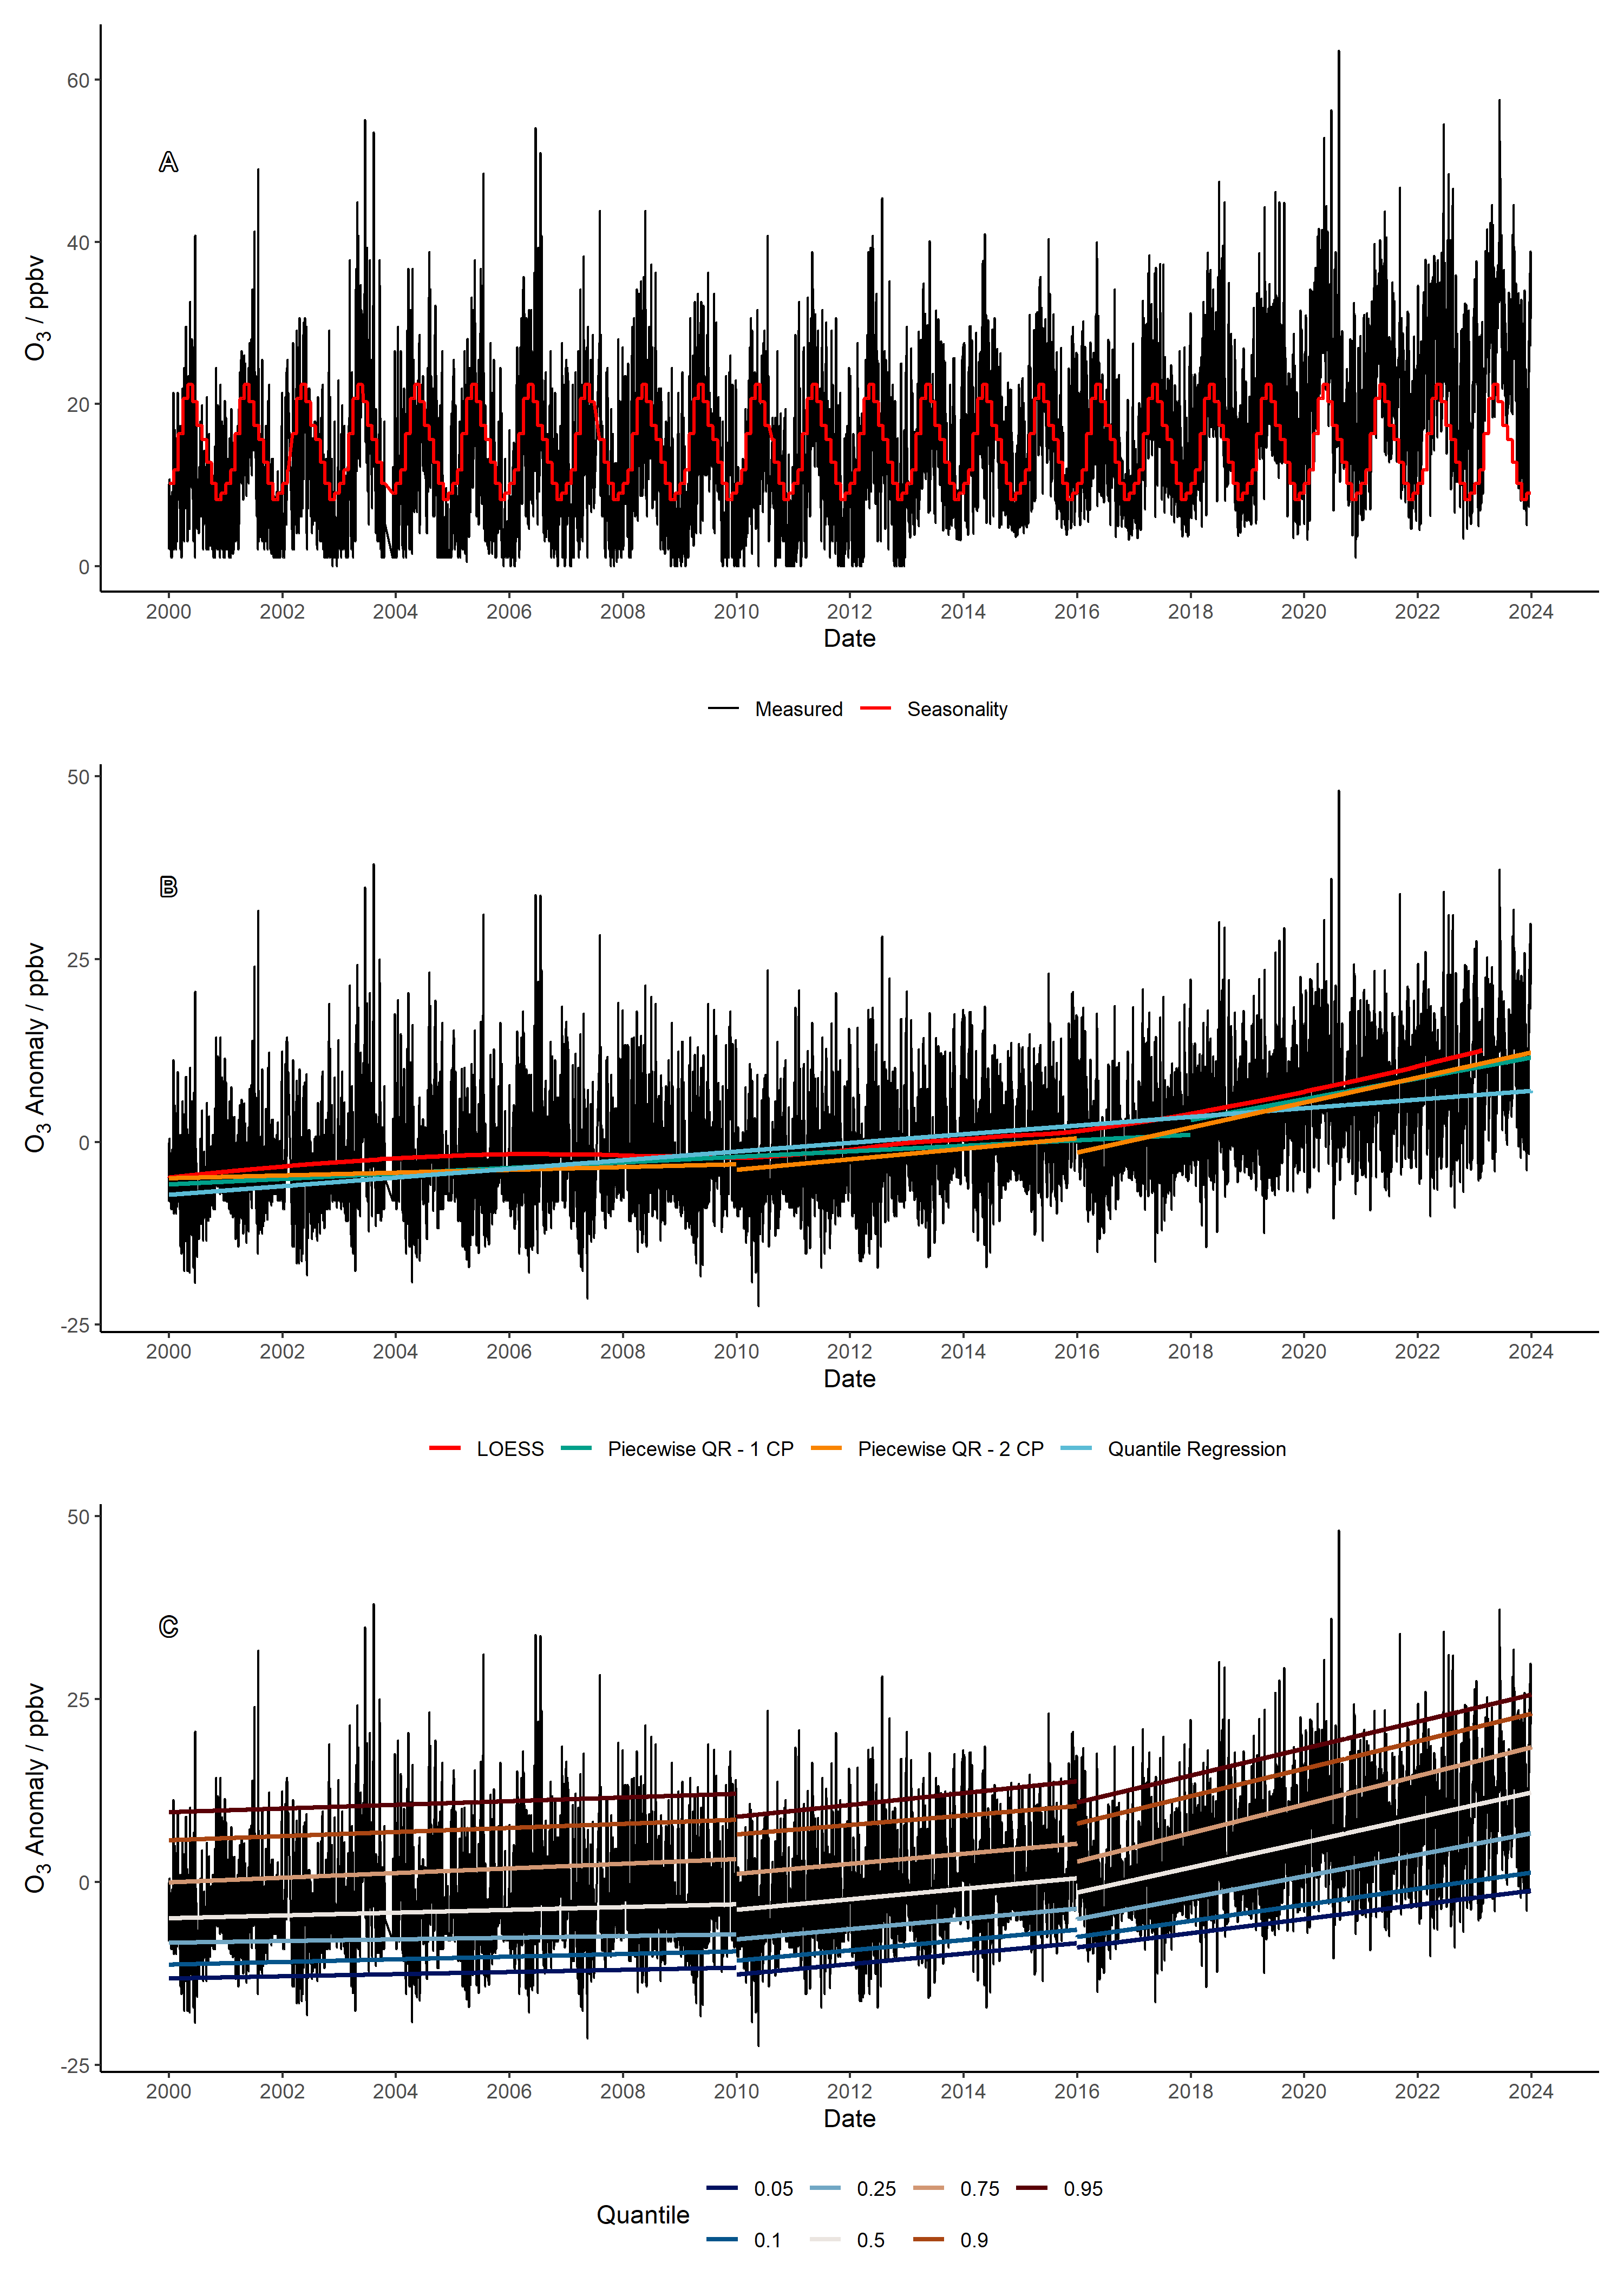
\includegraphics[width=12cm]{plots/method.png}
\caption{Example trend determination for an O3 time series (London Bloomsbury - GB0566A). A - O3 concentration time series and monthly median climatology. B - Anomaly time series (concentration minus climatology) and 4 trend options, LOESS, QR, PQR1 and PQR2. C - Anomaly time series and PQR2 across $\tau$ = 0.05, 0.10, 0.25, 0.50, 0.75, 0.95.}
\label{method_plot}
\end{figure*}

To determine what breakpoints to use on each time series, 109 scenarios per time series defined by 1, 2 or 3 QRs were created, with break points occurring on the 1st of January 2002 - 2022 and in the cases where there were 2 breakpoints, these could not occur within 5 years of each other. The cases with 2 or 3 regressions were combined into a single PQR, (PQR1, PQR2). All regressions were calculated at $\tau$ = 0.05, 0.10, 0.25, 0.50, 0.75, 0.95 and 0.95, and did not vary between segments of a piecewise regression.

To select ‘change points’ from the array of breakpoints available, the model performance was evaluated via Akaike information criterion (AIC). The piecewise scenario with the minimum AIC at $\tau$ = 0.5 were selected as the change points for a given time series. It is possible that the change points would vary with $\tau$, however, it was decided to only determine these at $\tau$ = 0.5 to allow comparison of the same change points across the various $\tau$ values. It would be increasingly difficult to draw conclusions if both $\tau$ and change points could vary within a time series.  Figure \ref{method_plot} demonstrates this process on a single timeseries. Change points could be assessed for their efficacy (i.e. is the effect of introducing a change point important) by comparing the QR and the best PQR1 and PQR2 cases, but as this does not substantively change the results presented here, this was not done and the PQR2 fits were determined to be the most appropriate in all cases.

\clearpage
\section{Results and Discussion}
The dataset that results from the application of this method has several degrees of freedom to bear in mind during discussion. For a given timeseries (one species at a one site) there are two break points that are common for all the trend lines, and as there are 7 quantiles that the slopes have been calculated for this results in 21 slopes, each with an associated p-value. When comparing between sites (or even species within a site) the breakpoints can differ. This is necessary to capture the changing trends observed at urban sites but does complicate describing them. For this discussion we have grouped the sites into those from Europe and those from the United States, though details on individual European countries are available in the SI. 
To aid in summarising, in some cases the results have been grouped into time periods of a few years – in these cases if a trend changes due to a break point both trends have been counted. For example, if between 2000 and 2004 a site were to go from increasing O3 to decreasing O3, this would be described as ‘between 2000 and 2004 there was one increasing O3 trend and one decreasing O3 trend’. In the case where a site had a break point in 2003, but the trend remained increasing, this will be counted as one increasing trend. This has the benefit that no one category can count more than then number of available time series. In visualisation, both trends would be shown.

Trends have been collated into significance categories: p $\le$ 0.05, 0.05 $<$ p $\le$ 0.10, 0.10 $<$ p $\le$ 0.33 and p > 0.33, slopes where the p-value is > 0.33 are generally treated as ‘no trend’ regardless of the magnitude (generally we observe that as the magnitude of the trend decreases so does its significance), though sometimes are given with a direction when required by a visualisation.

\subsection{Overview of Trends} \label{sect:overview_of_trends}
To begin with, the $\tau$ = 0.5 trends of O3 and NO2 were examined and are presented on maps in figures \ref{fig:arrow_eu_o3}, \ref{fig:arrow_us_o3}, \ref{fig:arrow_eu_no2} and \ref{fig:arrow_us_no2}.

\begin{figure*}[htbp]
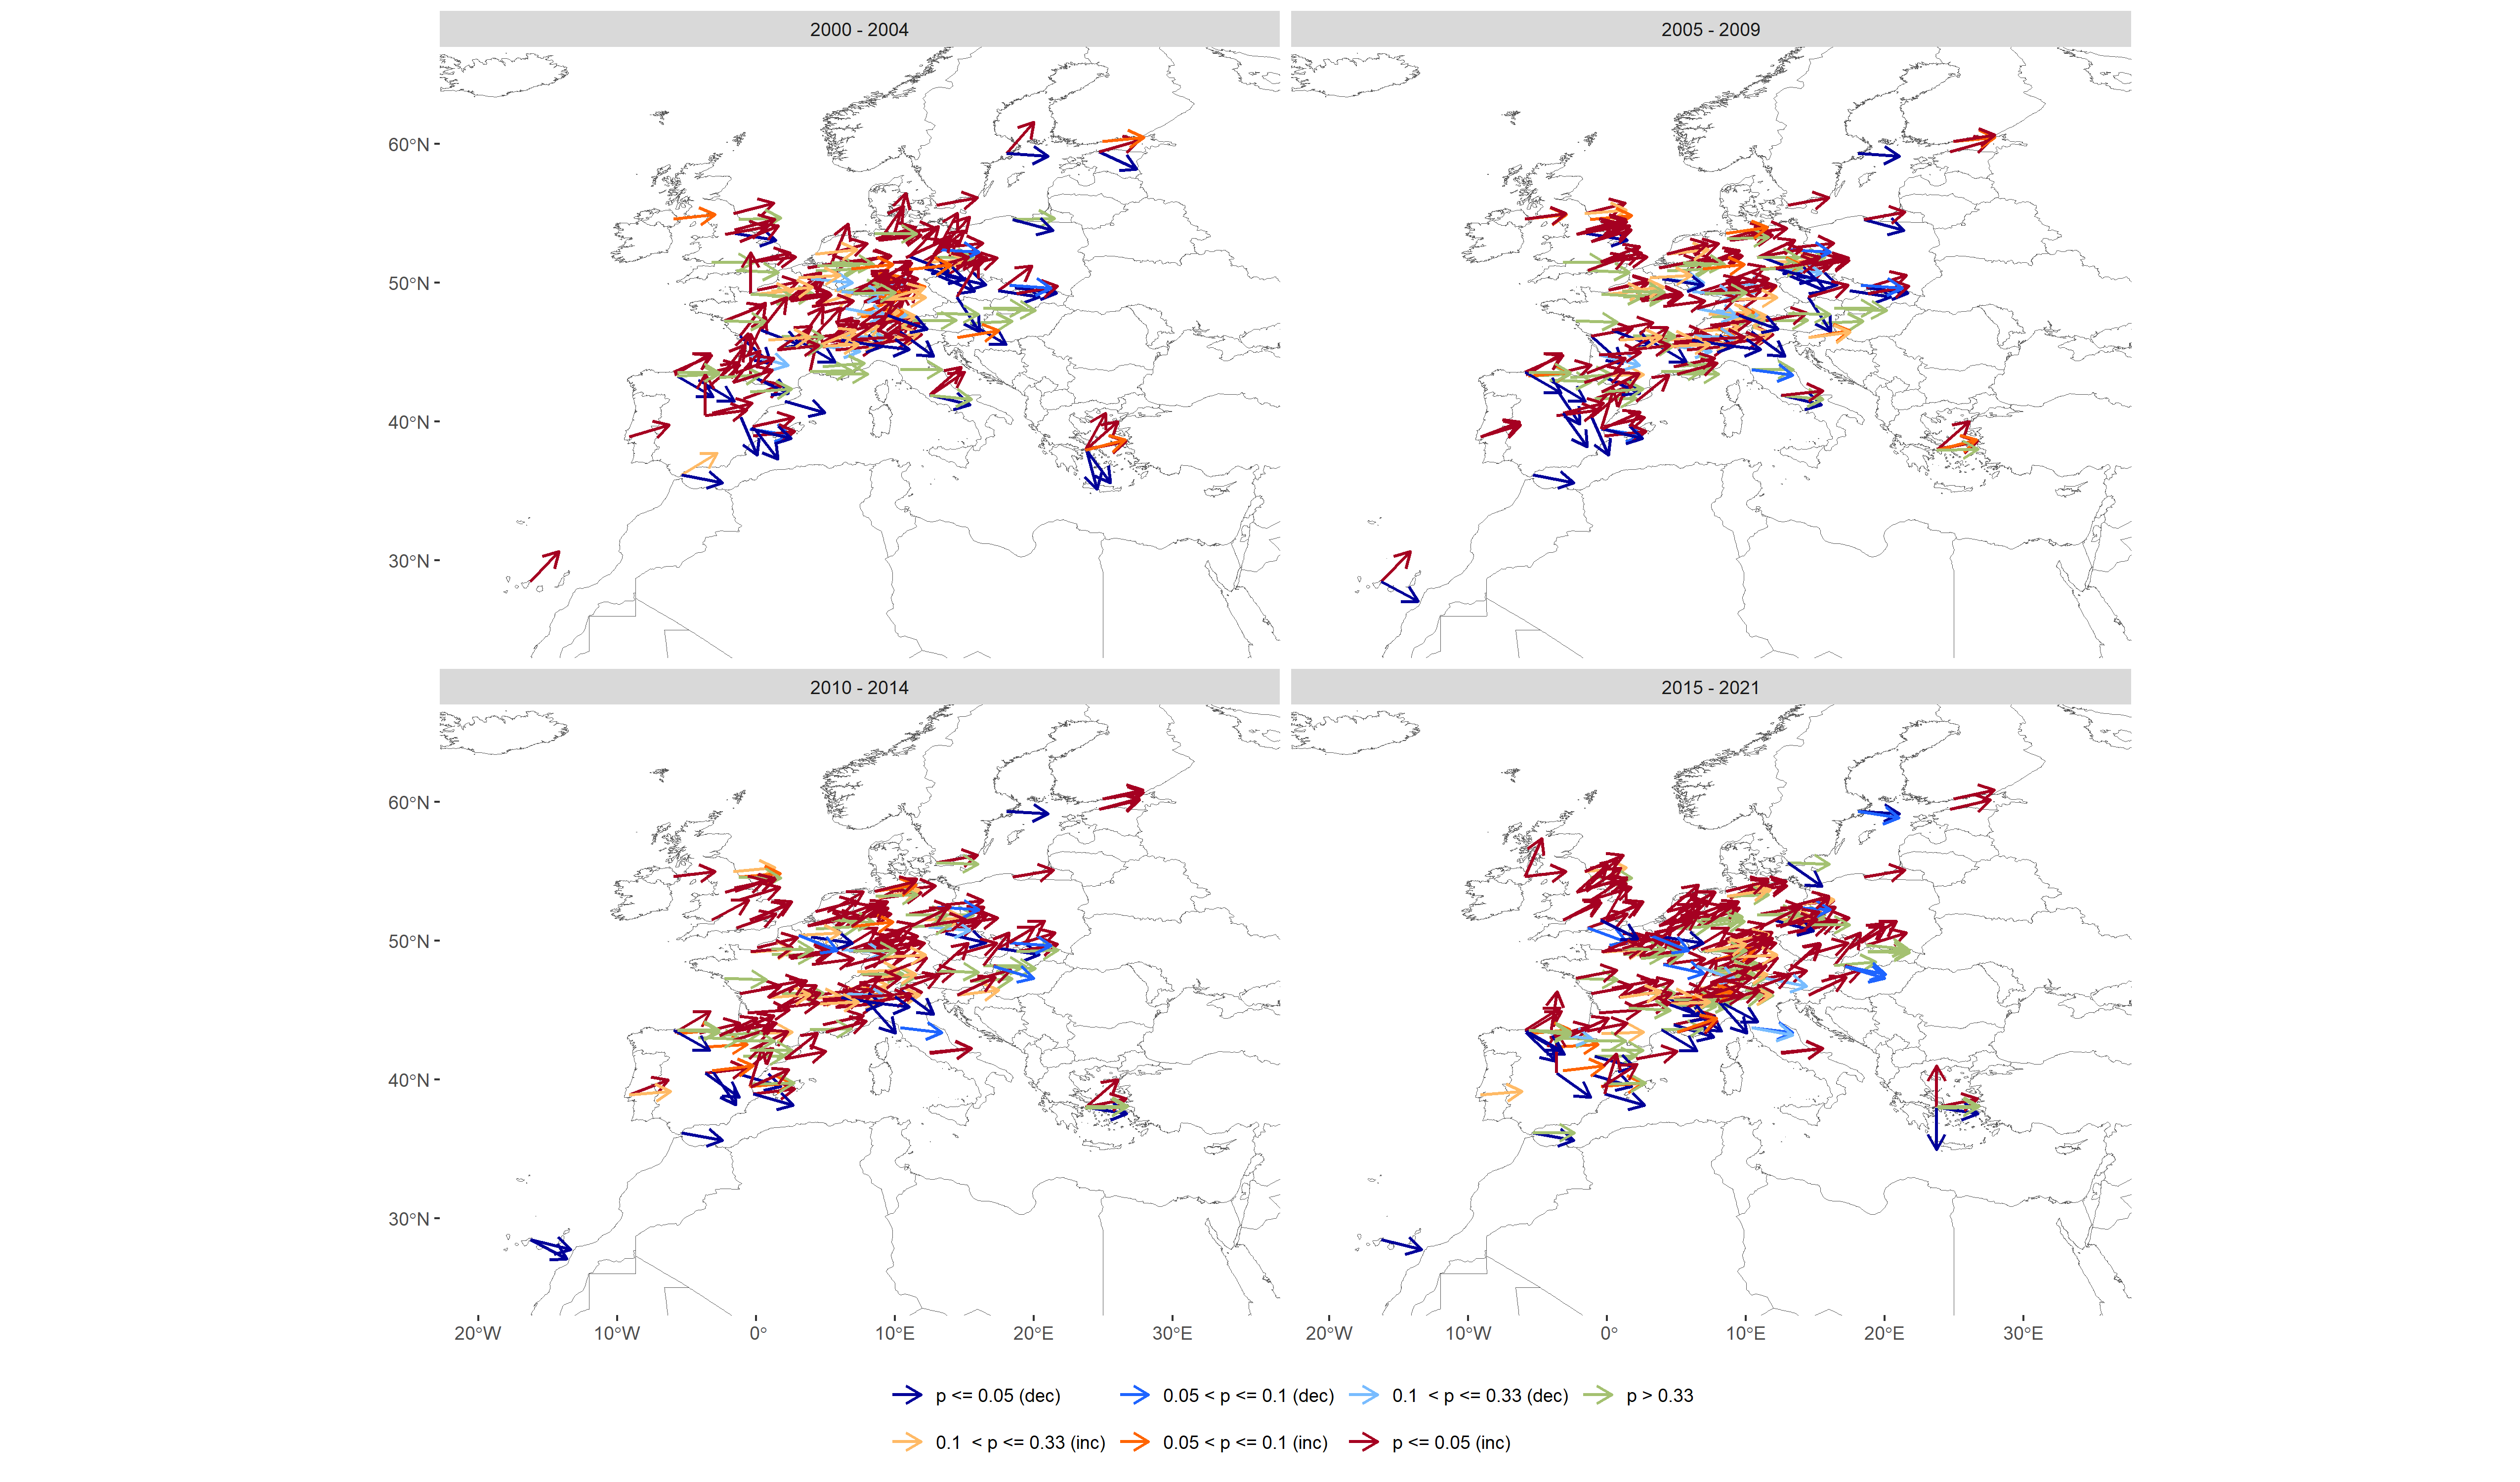
\includegraphics[width=12cm]{plots/arrow_maps/o3/11/EU_map_spc_o3_tau_0.5_seg_11_14.png}
\caption{}
\label{fig:arrow_eu_o3}
\end{figure*}

\begin{figure*}[htbp]
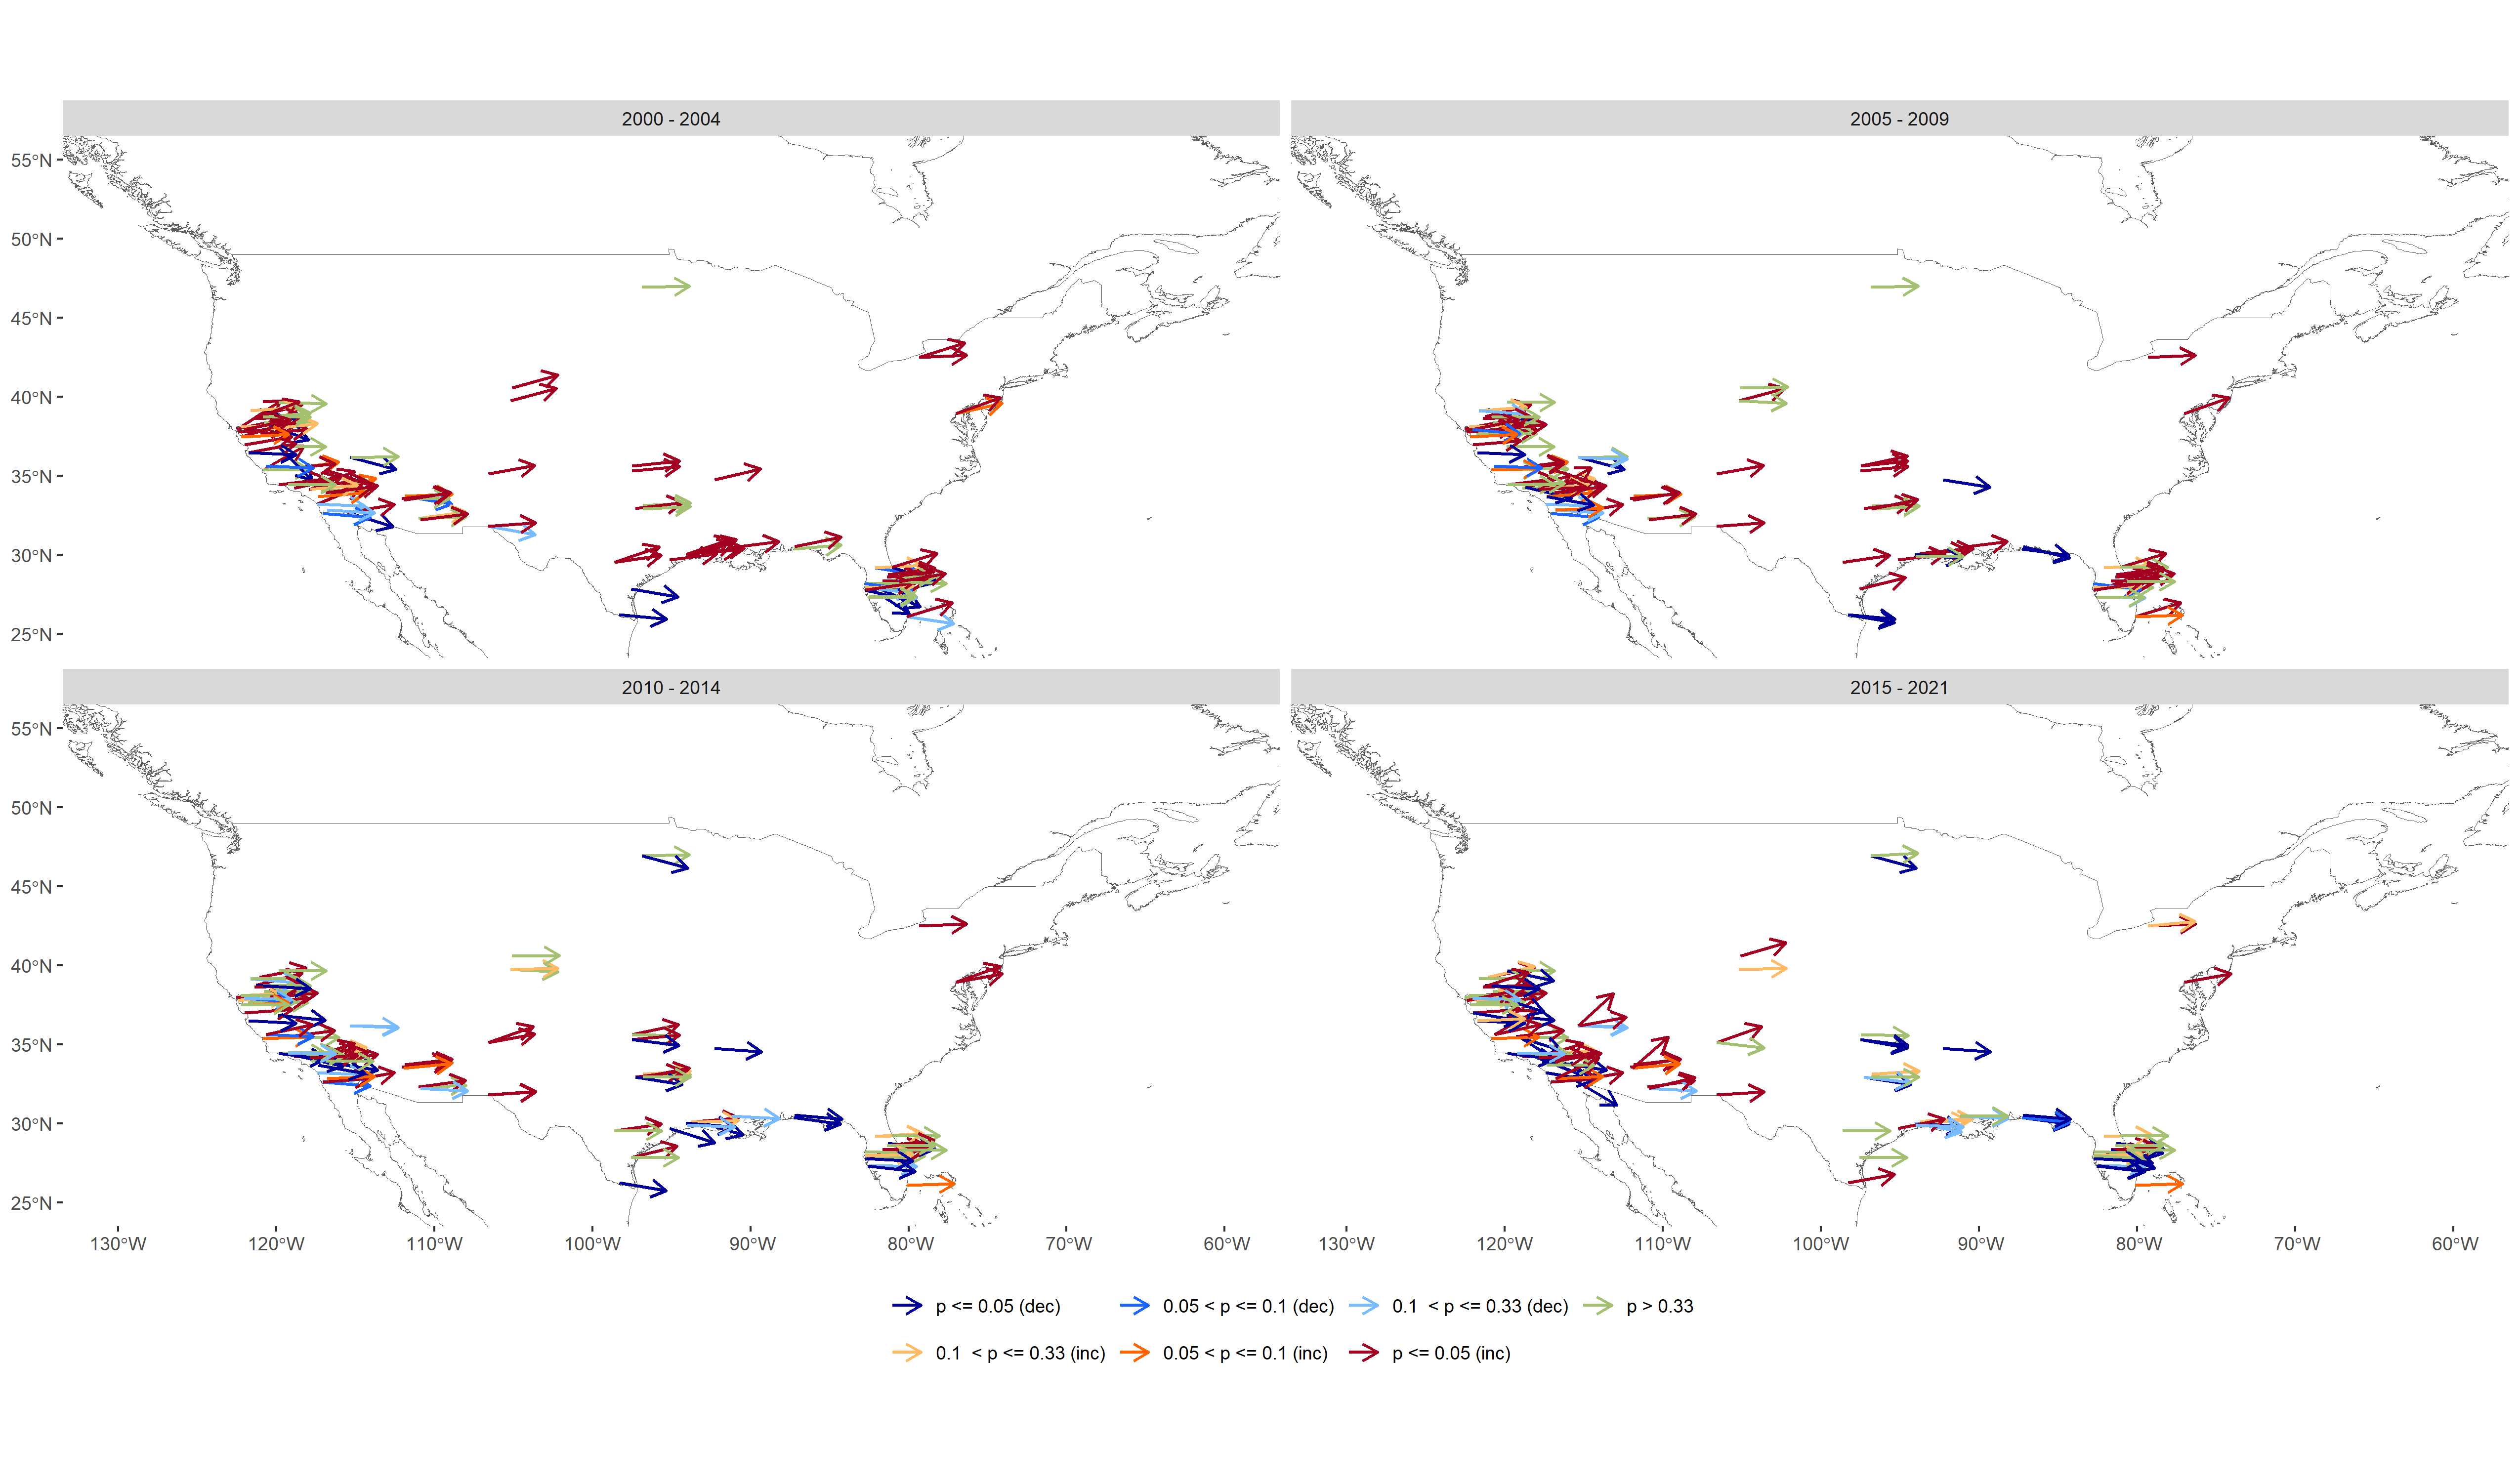
\includegraphics[width=12cm]{plots/arrow_maps/o3/11/US_map_spc_o3_tau_0.5_seg_11_14.png}
\caption{}
\label{fig:arrow_us_o3}
\end{figure*}

\begin{figure*}[htbp]
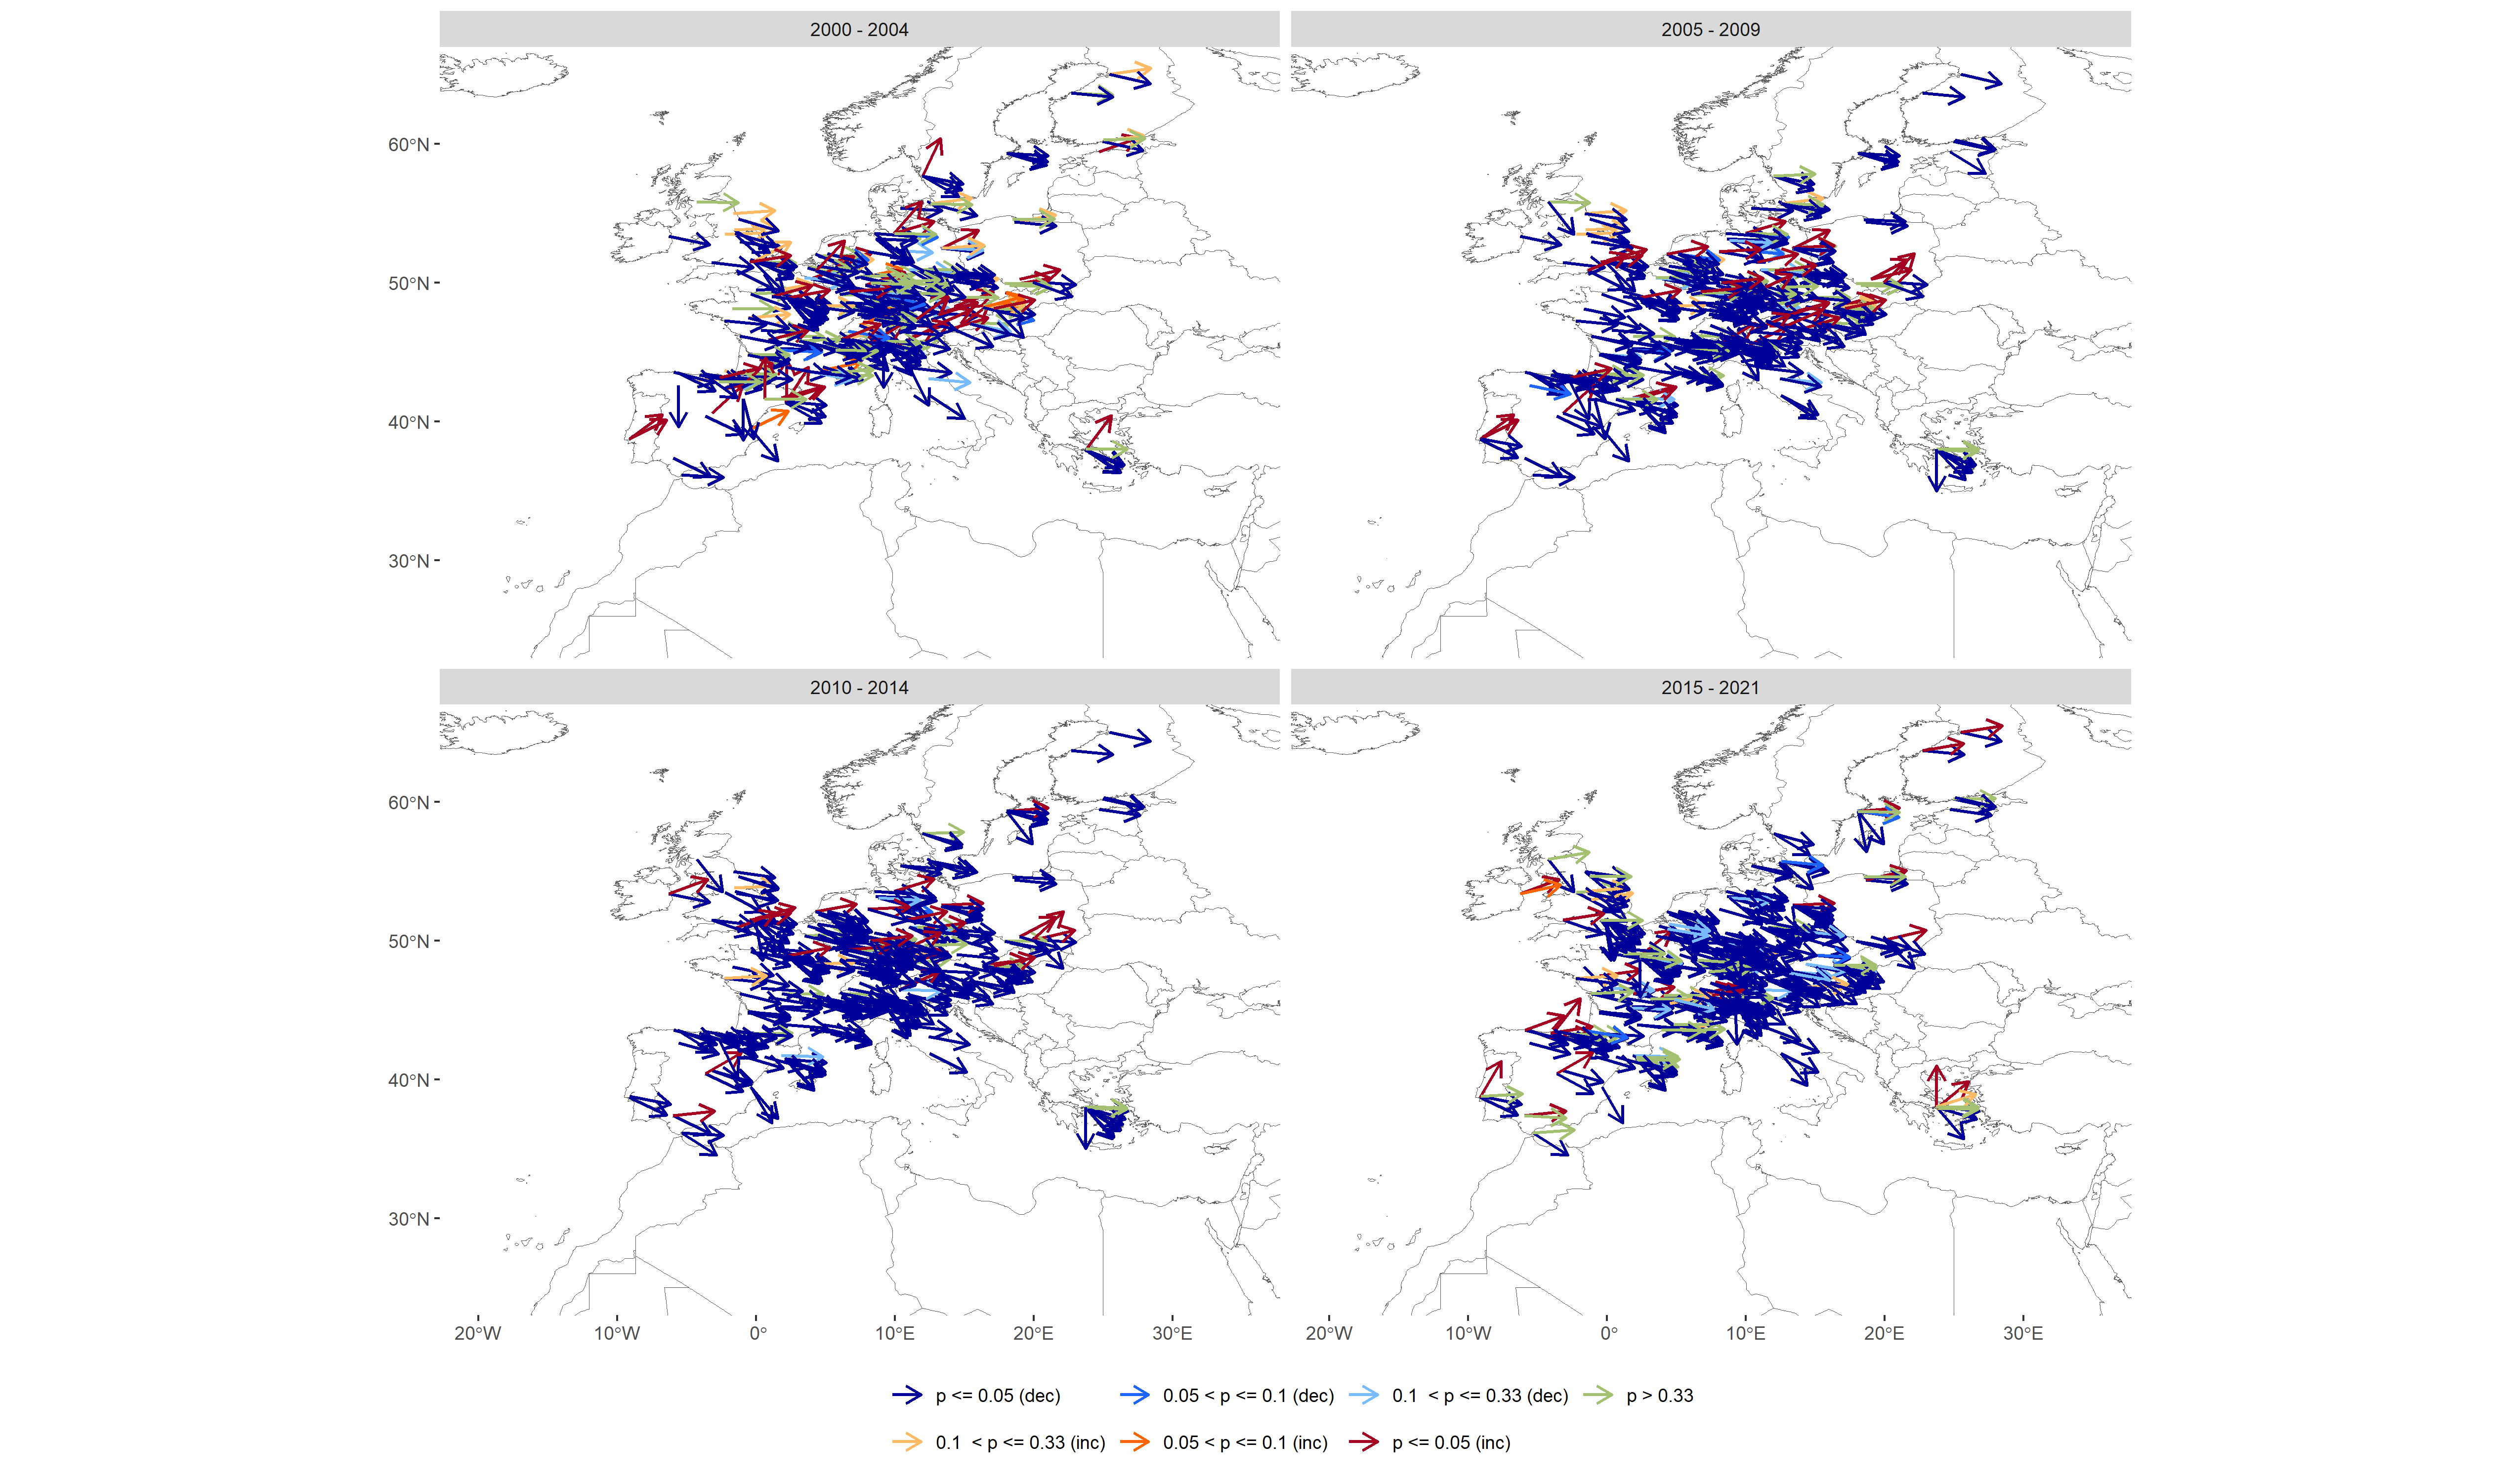
\includegraphics[width=12cm]{plots/arrow_maps/no2/11/EU_map_spc_no2_tau_0.5_seg_11_14.png}
\caption{}
\label{fig:arrow_eu_no2}
\end{figure*}

\begin{figure*}[htbp]
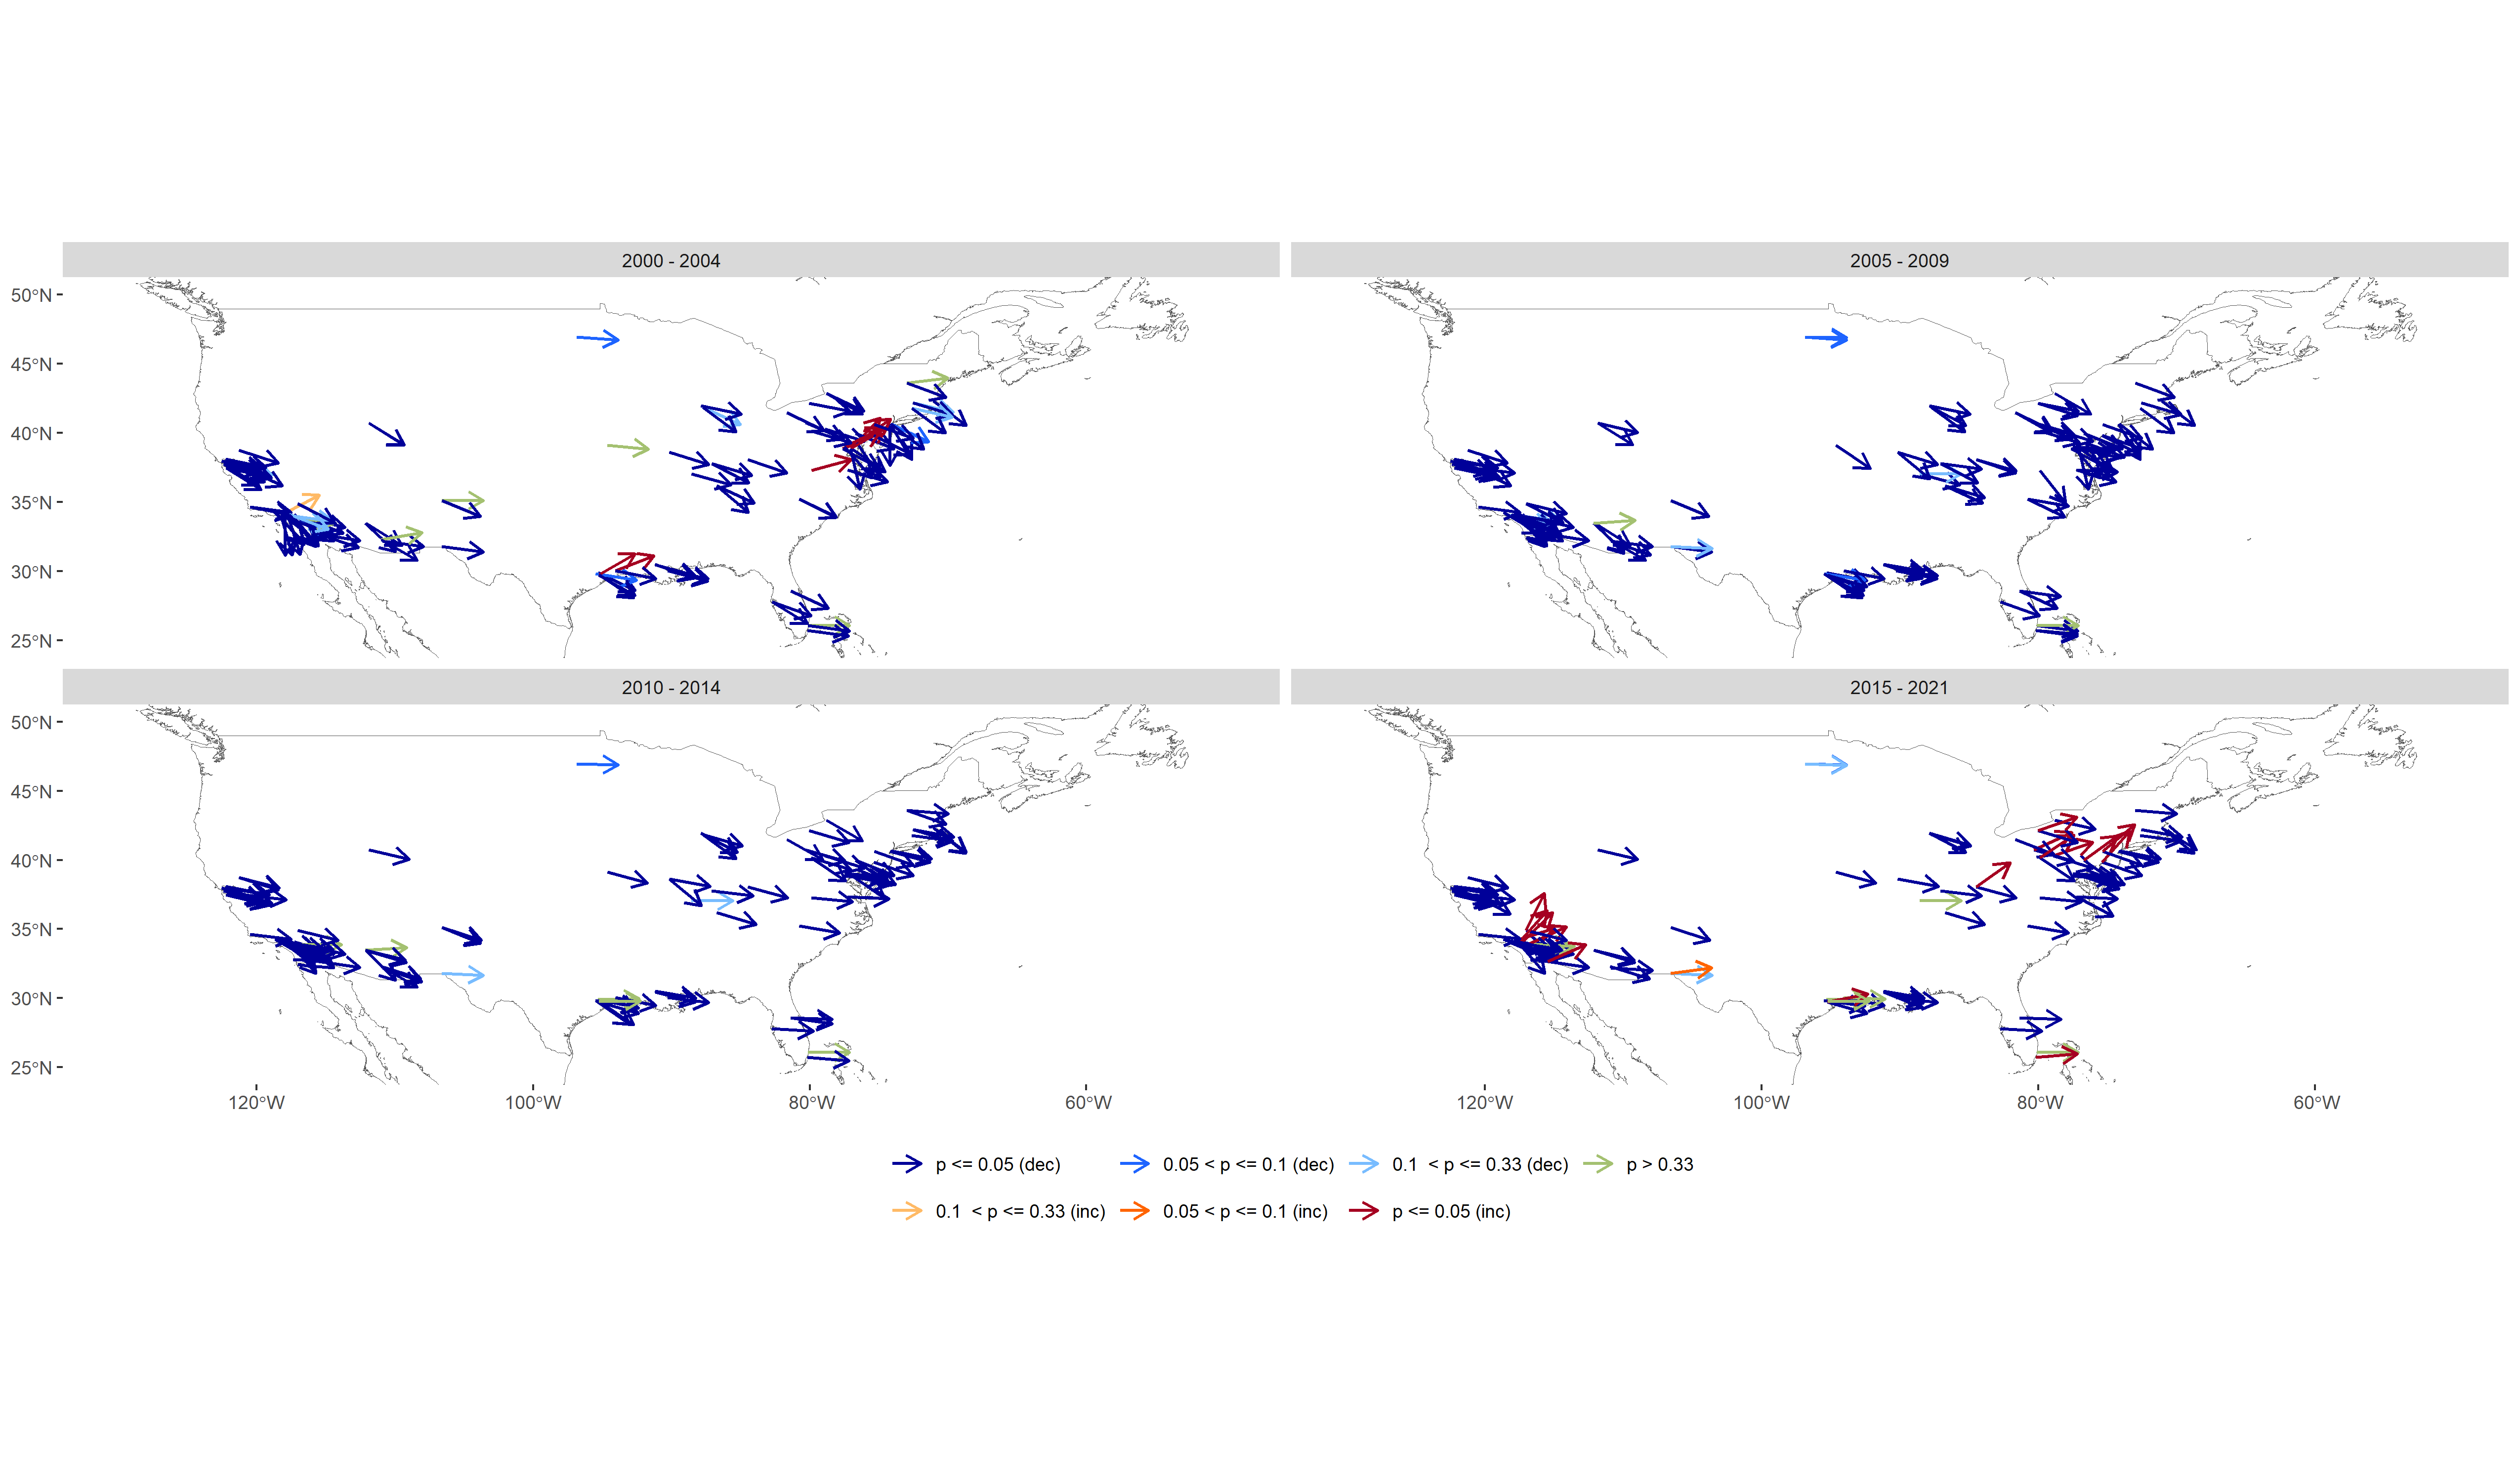
\includegraphics[width=12cm]{plots/arrow_maps/no2/11/US_map_spc_no2_tau_0.5_seg_11_14.png}
\caption{}
\label{fig:arrow_us_no2}
\end{figure*}

In Europe, between 2000 and 2004 there were 108 trends where O3 was increasing, and 41 where it was decreasing, 32 showed no trend. By 2015-2021 123 had an increasing trend, 32 decreasing and 41 with no trend, indicating generally increasing O3 concentrations across Europe. This is somewhat mirrored by the trends in NO2, where in 2000-2004 69 trends where increasing, 182 decreasing and 59 with no trend, changing to 30 increasing, 241 decreasing and 39 with no trend by 2015-2021. This is commensurate with the general picture that urban locations in Europe are still on the VOC limited portion of the O3 production isopleth, and decreasing NOx increases O3 production. 
This contrasts with the USA, were in 2000-2004, there were 10 sites with increasing NO2, but 0 sites increasing between 2005 and 2014, but in 2015 -2021 17 sites had begun increasing in NO2 again – though notably as seen from figure CC these are different sites to those that were increasing at the beginning of the century. This increase in NO2 is not clearly reflected by the O3 trends with 62 / 23 / 22 increasing / decreasing / no trend in 2000 – 2004 and 44 / 34 / 25 increasing / decreasing / no trend, with a decreasing number of sites O3 with a positive trend in O3, suggesting that the majority of decreasing NO2 trends are slowing the increase in O3. The counts of sites at all values of $\tau$ can be found in tables \ref{table:europe_slope_segs} and \ref{table:usa_slope_segs}. 
For O3 in Europe, at sites with increasing trends the median slope was 0.36 ppbv yr-1, slightly lower than in the US, where they were increasing by 0.40 ppbv yr-1. For NO2, the median rate of increase was the same in Europe 0.36 ppbv yr-1, but higher at 0.71 ppbv yr-1 in the US. For decreasing trends, O3 and NO2 in Europe and the US were all similar, O3 in Europe decreasing at -0.40 ppb yr-1, (-0.36 ppbv yr-1) in the US and for NO2 -0.39 ppbv yr-1 in Europe and -0.47 in the US. This information along with the 5 th and 95 th percentile (still at $\tau$ = 0.5) are shown in table \ref{table:slope_ranges}. 




\input{tables/slope_ranges.txt}

\input{tables/europe_segs_11_14.txt}

\input{tables/usa_segs_11_14.txt}

\subsubsection{Significance of Trends}

\begin{figure*}[htbp]
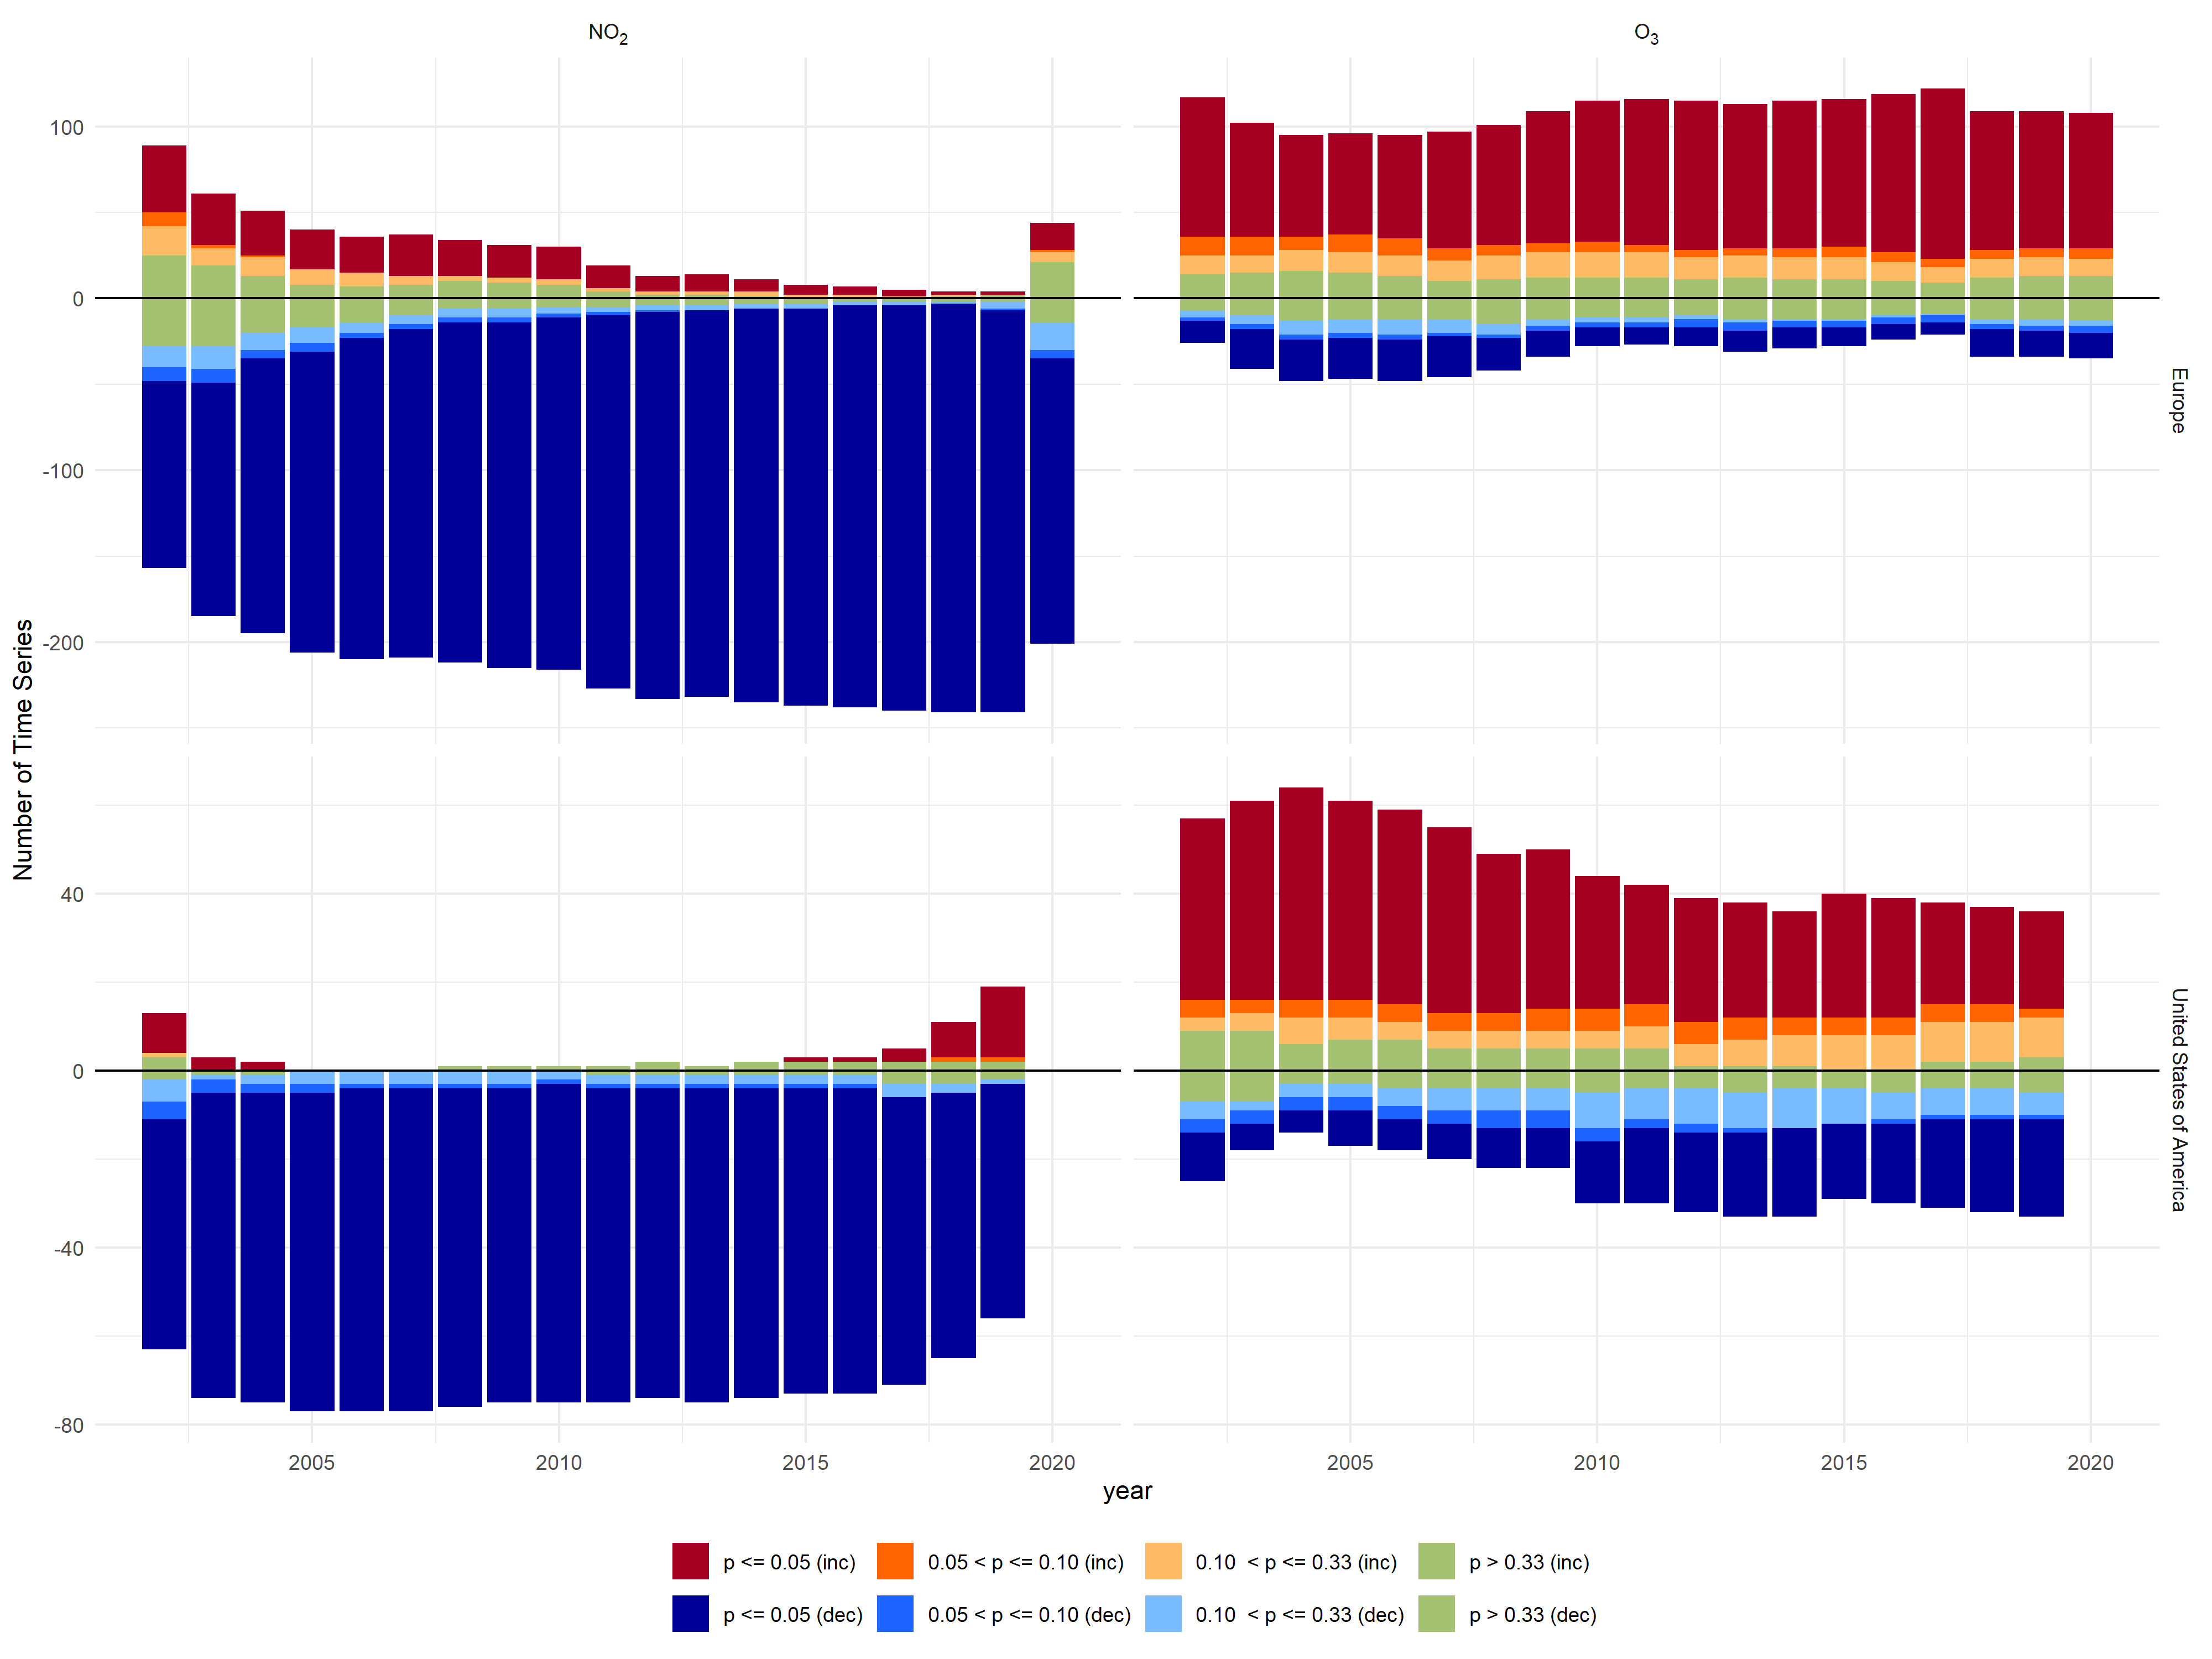
\includegraphics[width=12cm]{plots/p_bar_year.png}
\caption{}
\label{fig:p_bar_year}
\end{figure*}

Figure \ref{fig:p_bar_year} counts the trends by significance group and direction per year. This reveals the majority of trends are positive or negative with high certainty. It also reinforces the observations from section \ref{sect:overview_of_trends}, where both Europe and the US see O3 increasing at number of sites, with there being proportionally more sites with a decreasing trend in the US. This additionally shows that the number of high certainty decreasing trends in O3 has been present since ~2010, joined by a slow decline in increasing trends. 

In NO2 the feature of some sites beginning to show increasing trends in the US is clear, with this pattern beginning in 2015-2016. Between 2000 and 2019 Europe nearly moved all sites to a trend of decreasing NO2, however, this reversed for several sites in 2020. This signal will be present in the data due to the reduction in NO2 concentrations in Europe which were a side effect of public health measures REF Lee 2020, Grange 2021, (also maybe Sokhi). The removal of these measures lead to an increase in NO2 as normal activities resumed, resulting in a positive trend in NO2 concentrations. There is not yet enough data for this method to capture a return to previous trends as change points were not allowed within 3 years of the end of the timeseries, so that there is sufficient data to perform the QR. For this reason 2000, 2001 and 2021 onward in Europe and 2000, 2001, 2020 and 2021 onwards for the USA were excluded from this year on year analysis, as it is not possible to capture changing trends in these regions. 



\subsection{Distribution of Change points}

\subsection{Trends Across Quantiles}

To investigate how the trends in urban ozone are generally changing over time in Europe and the USA, the distribution of slopes in each region was determined for each value of $\tau$. The distribution at the start (year = 2000) and end (year = 2019) of the 20-year period was compared (Figure \ref{o3_ridge_plot}). Generally, across all taus, the spread of the slope distributions in o3 was greater in 2000 compared with 2019. This is particularly true for Europe, where a clear reduction in the higher o3 slopes is observed between 2000 and 2019. For $\tau$ = 0.95, a much larger proportion of the slopes were > 1.25 ppbV yr-1 in 2000 than 2019. For $\tau$ = 0.95 in the USA, there is a reduction in the number of slopes with very negative (< 1.00 ppbV yr-1) slopes between 2000 and 2019.

\begin{figure*}[h!]
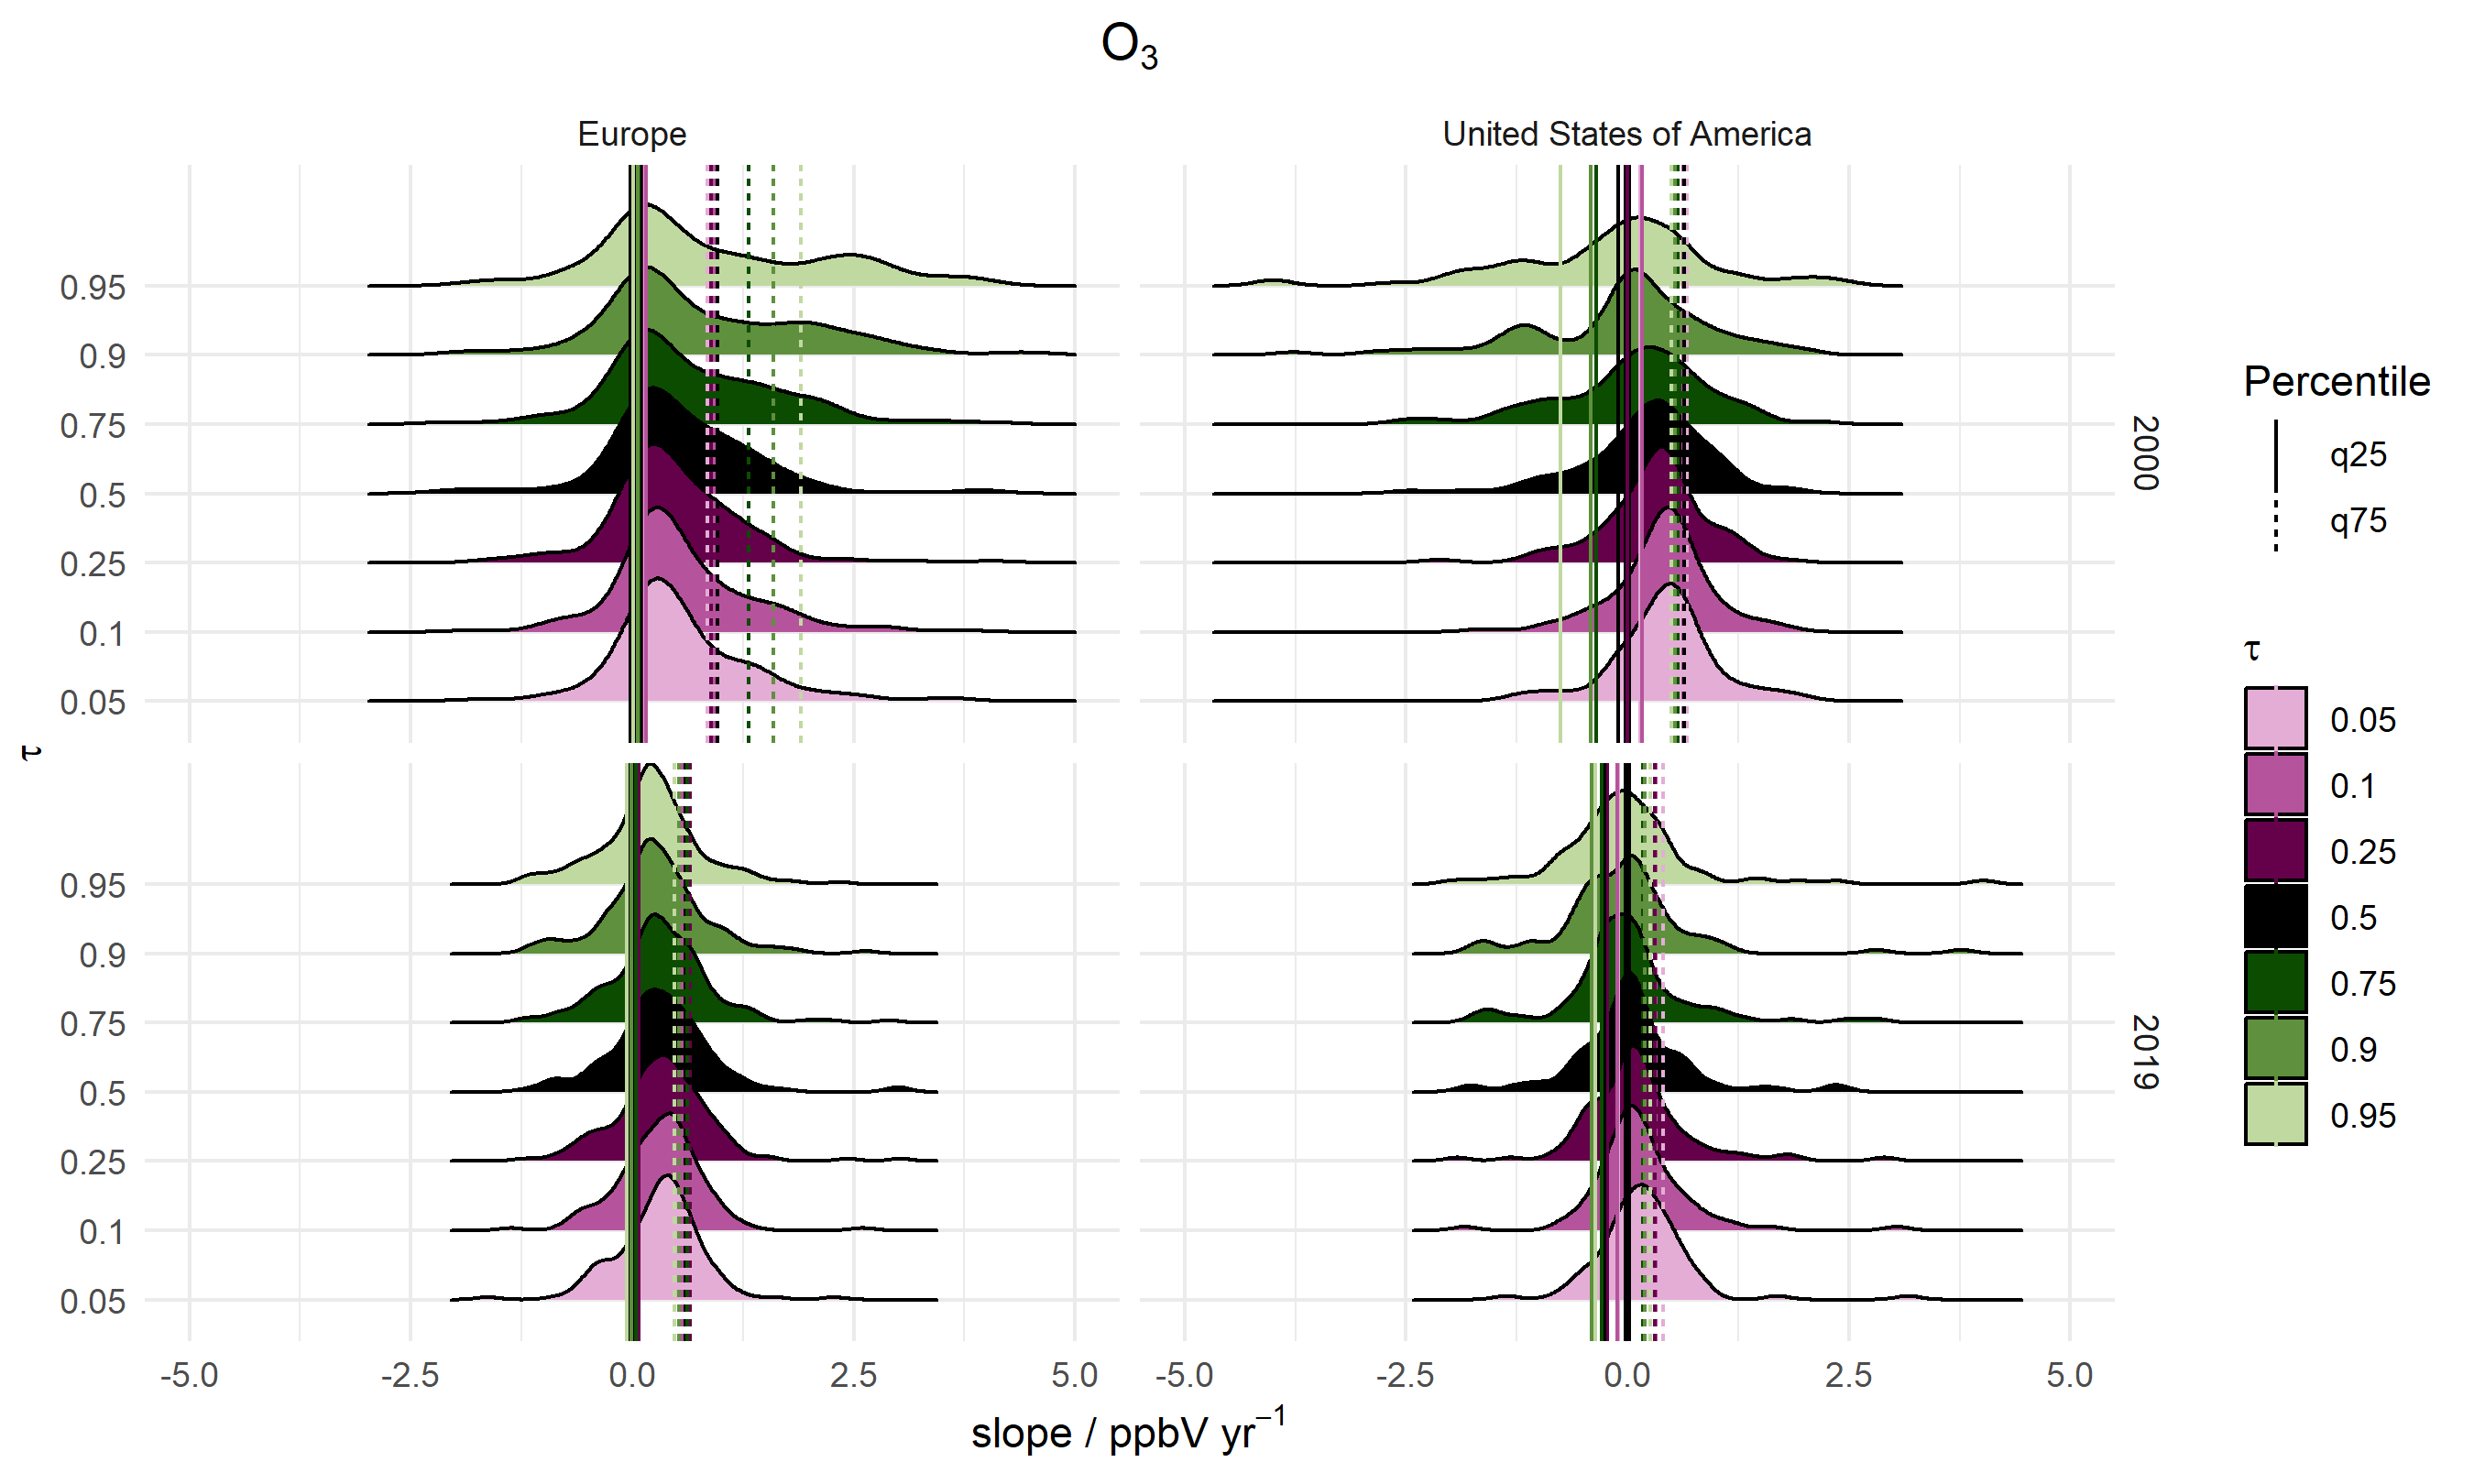
\includegraphics[width=12cm]{plots/o3_density_ridges_by_tau_continent_2000_2019.png}
\caption{}
\label{o3_ridge_plot}
\end{figure*}

In Europe, the bulk value of the slopes becomes more negative across all $\tau$ values (Figure \ref{no2_ridge_plot}). However, in the USA, despite the majority of slopes being negative in both 2000 and 2019, there is still a proportion of slopes with positive slopes in 2019, not observed in the European distribution. This is particularly true for 0.5 >= $\tau$ <= 0.9. The spread of the slope distributions was comparable between 2000 and 2019 for Europe, but smaller for the USA in 2019 compared to 2000.

\begin{figure*}[h!]
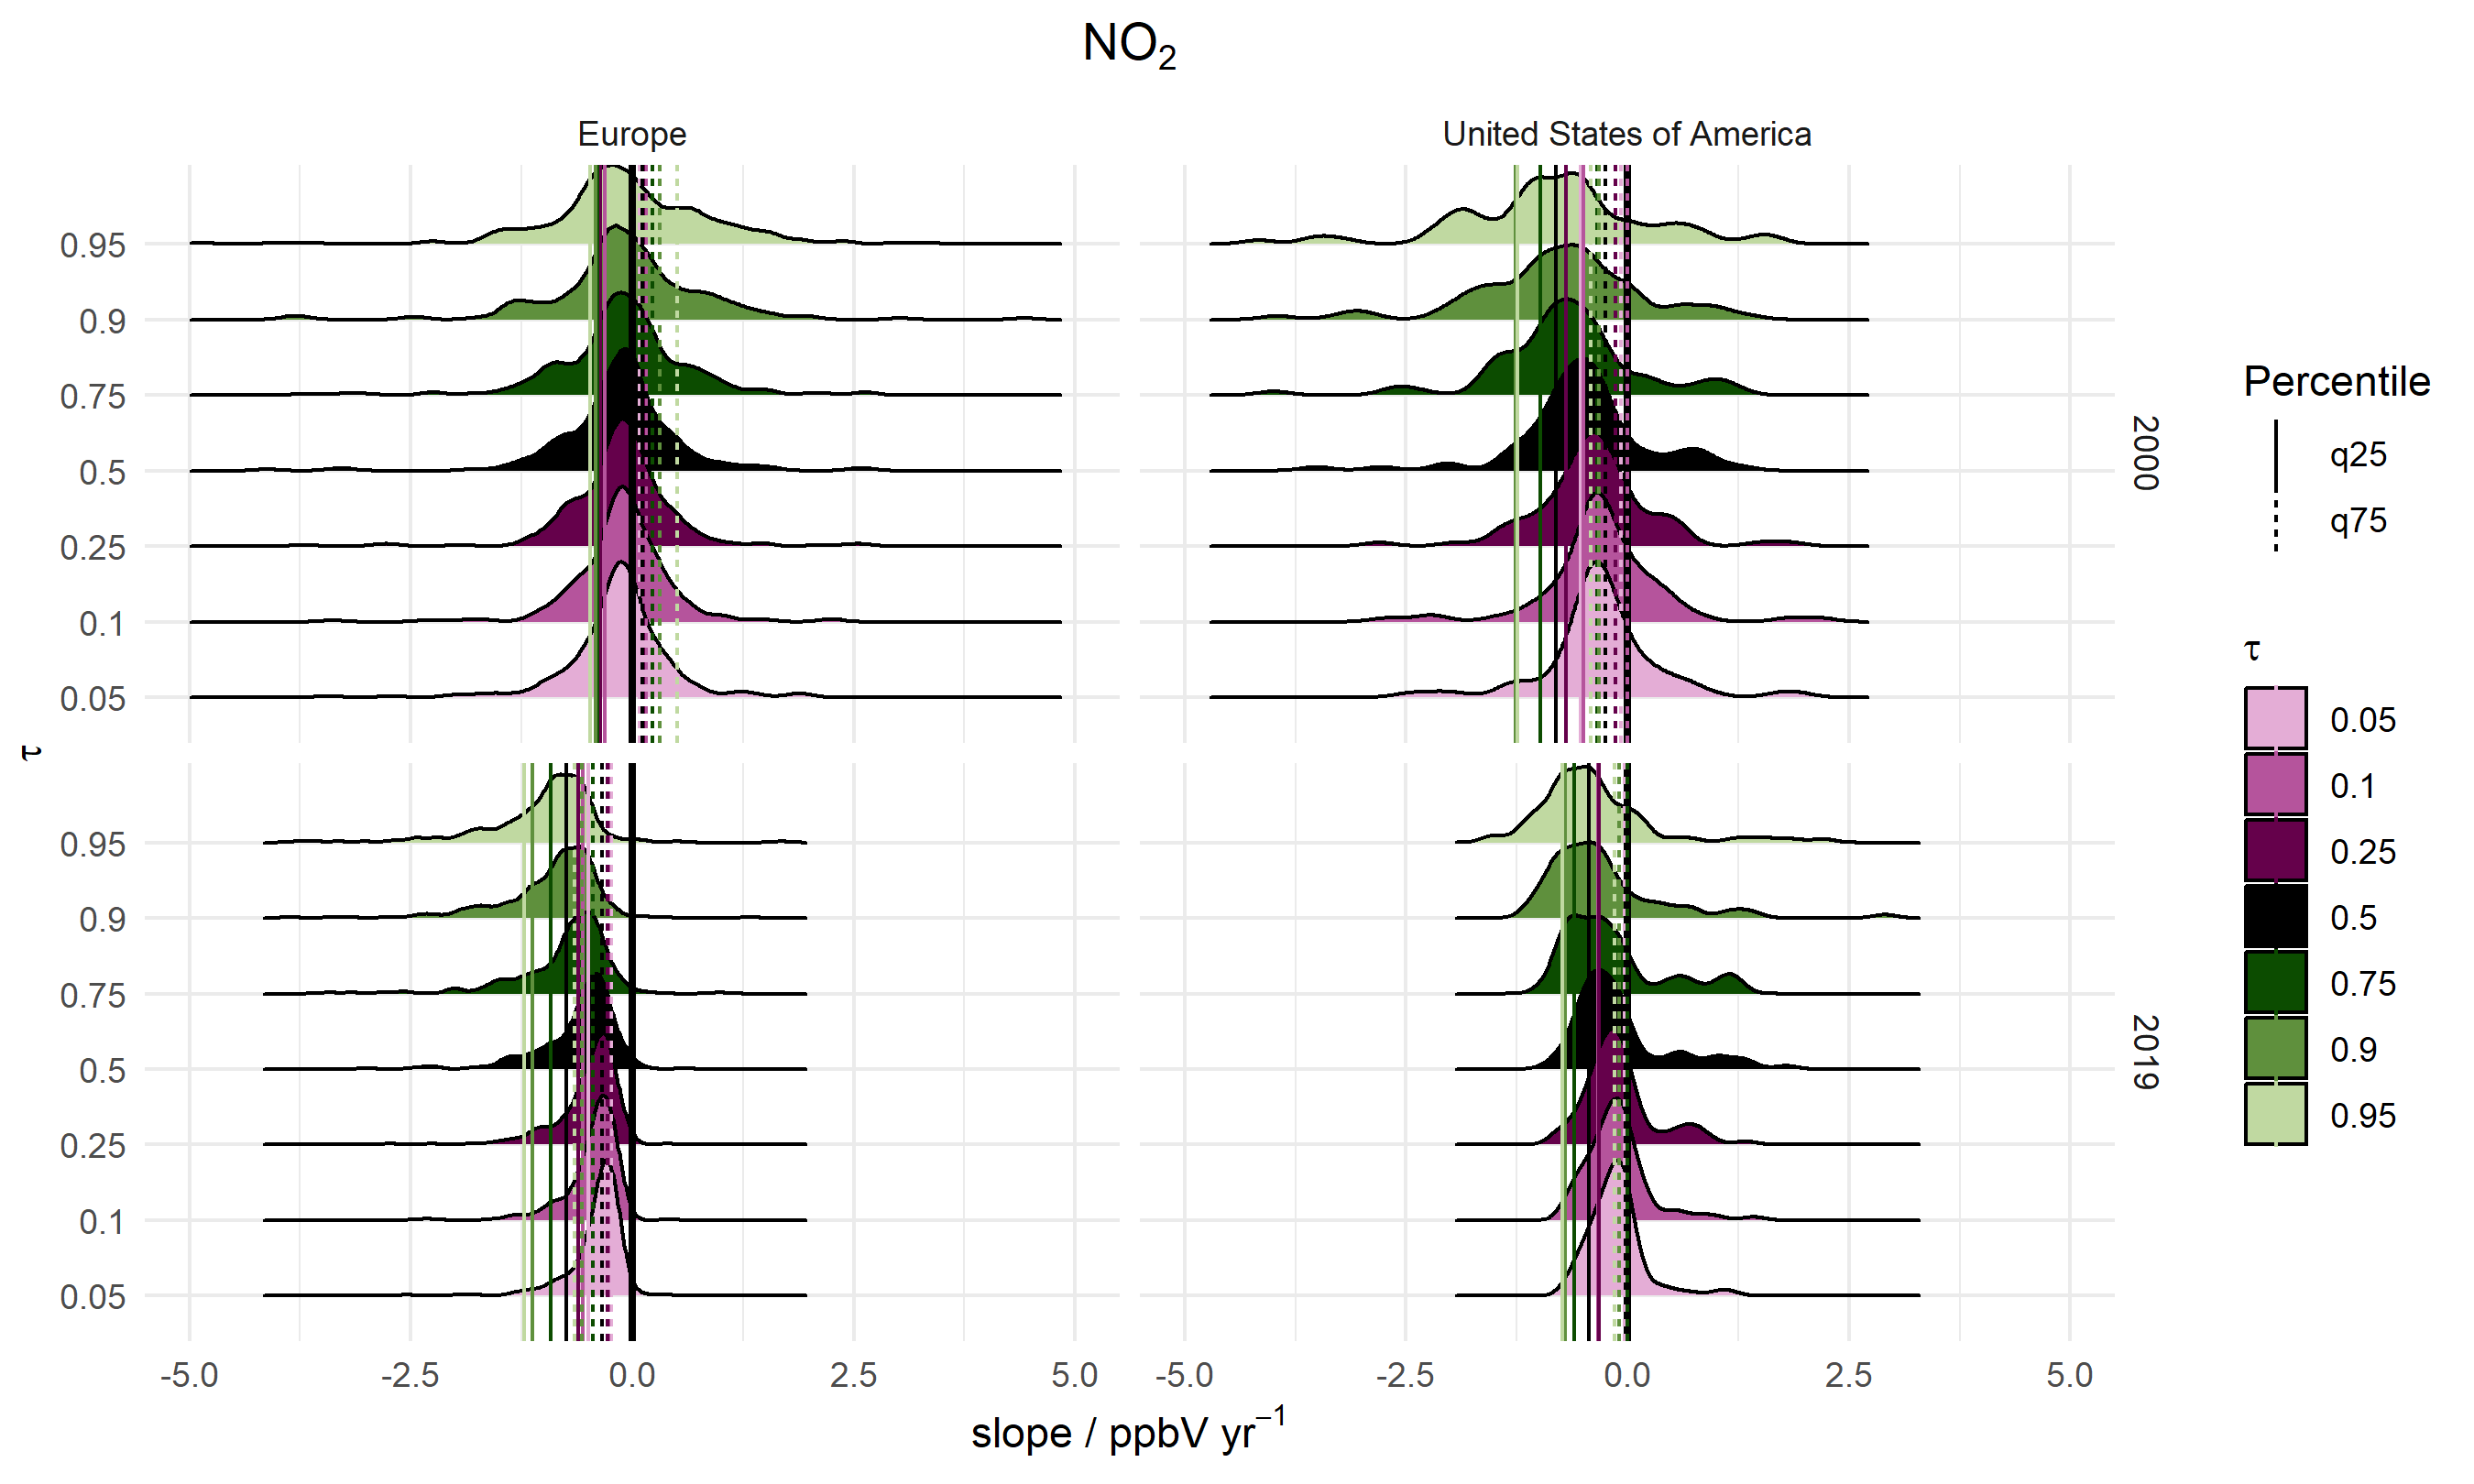
\includegraphics[width=12cm]{plots/no2_density_ridges_by_tau_continent_2000_2019.png}
\caption{}
\label{no2_ridge_plot}
\end{figure*}

Trends in the 5 th, 10 th, 25 th, 50 th, 75 th, 90 th and 95 th $\tau$ values were used to evaluate how urban ozone, and its trends, changed across Europe and the USA between 2000 and 2021. For both Europe and the USA, the median slope of the trendline for all sites was taken for each percentile. Using this analysis, Figure \ref{median_slopes_per_tau_cont_name_absolute} shows the resulting change in median no2, o3 and ox mixing ratios since 2000. Figure \ref{median_slopes_per_tau_cont_name_trends} describes how the magnitude and direction of the trendline changes annually.

In both Europe and the USA, median O3 mixing ratios have generally increased between 2000 and 2021 (middle panel, Figure \ref{median_slopes_per_tau_cont_name_absolute}). This is most clearly observed in Europe, where all percentiles demonstrated a consistent increase in median O3 across the two decades. Larger increases in O3 were observed in the lower percentile cases (+5.4 ppb, 5th percentile) compared to the higher percentiles (+3.5 ppb, 95th percentile), indicating that the lowest ambient O3 levels are increasing more rapidly than higher levels.  The picture is more mixed in the USA. Similarly to Europe, the largest increases in median O3 since 2000 were observed in the lower percentiles (+4.3 ppb, 5th percentile). In the 50th percentile case, median O3 increased to ca. +1.8 ppb by 2011 before plateauing between 2011 and 2021, with a similar pattern also observed in the 75th percentile case (+1.1 ppb up to 2009, then plateauing). In both cases, an uptick is observed from 2019, with an overall vicennial increase in o3 of +2.0 ppb (50th percentile) +1.2 ppb (75th percentile). In contrast, in the highest percentile cases, median O3 was lower in 2021 than in 2001 (-0.18 and -0.19 ppb, 90th and 95th percentiles respectively). This suggests that higher ambient levels of O3 have reduced in magnitude since 2000, compared to lower ambient levels which are continuing to increase. In both Europe and the USA, median ambient NO2 mixing ratios have reduced, with the largest reductions observed in the 95th percentile case (-11.6 ppb and -14.6 ppb for Europe and the USA respectively). Smaller reductions were observed in the 5th percentile case (-4.5 and -5.4 ppb for Europe and the USA respectively).

\begin{figure*}[h!]
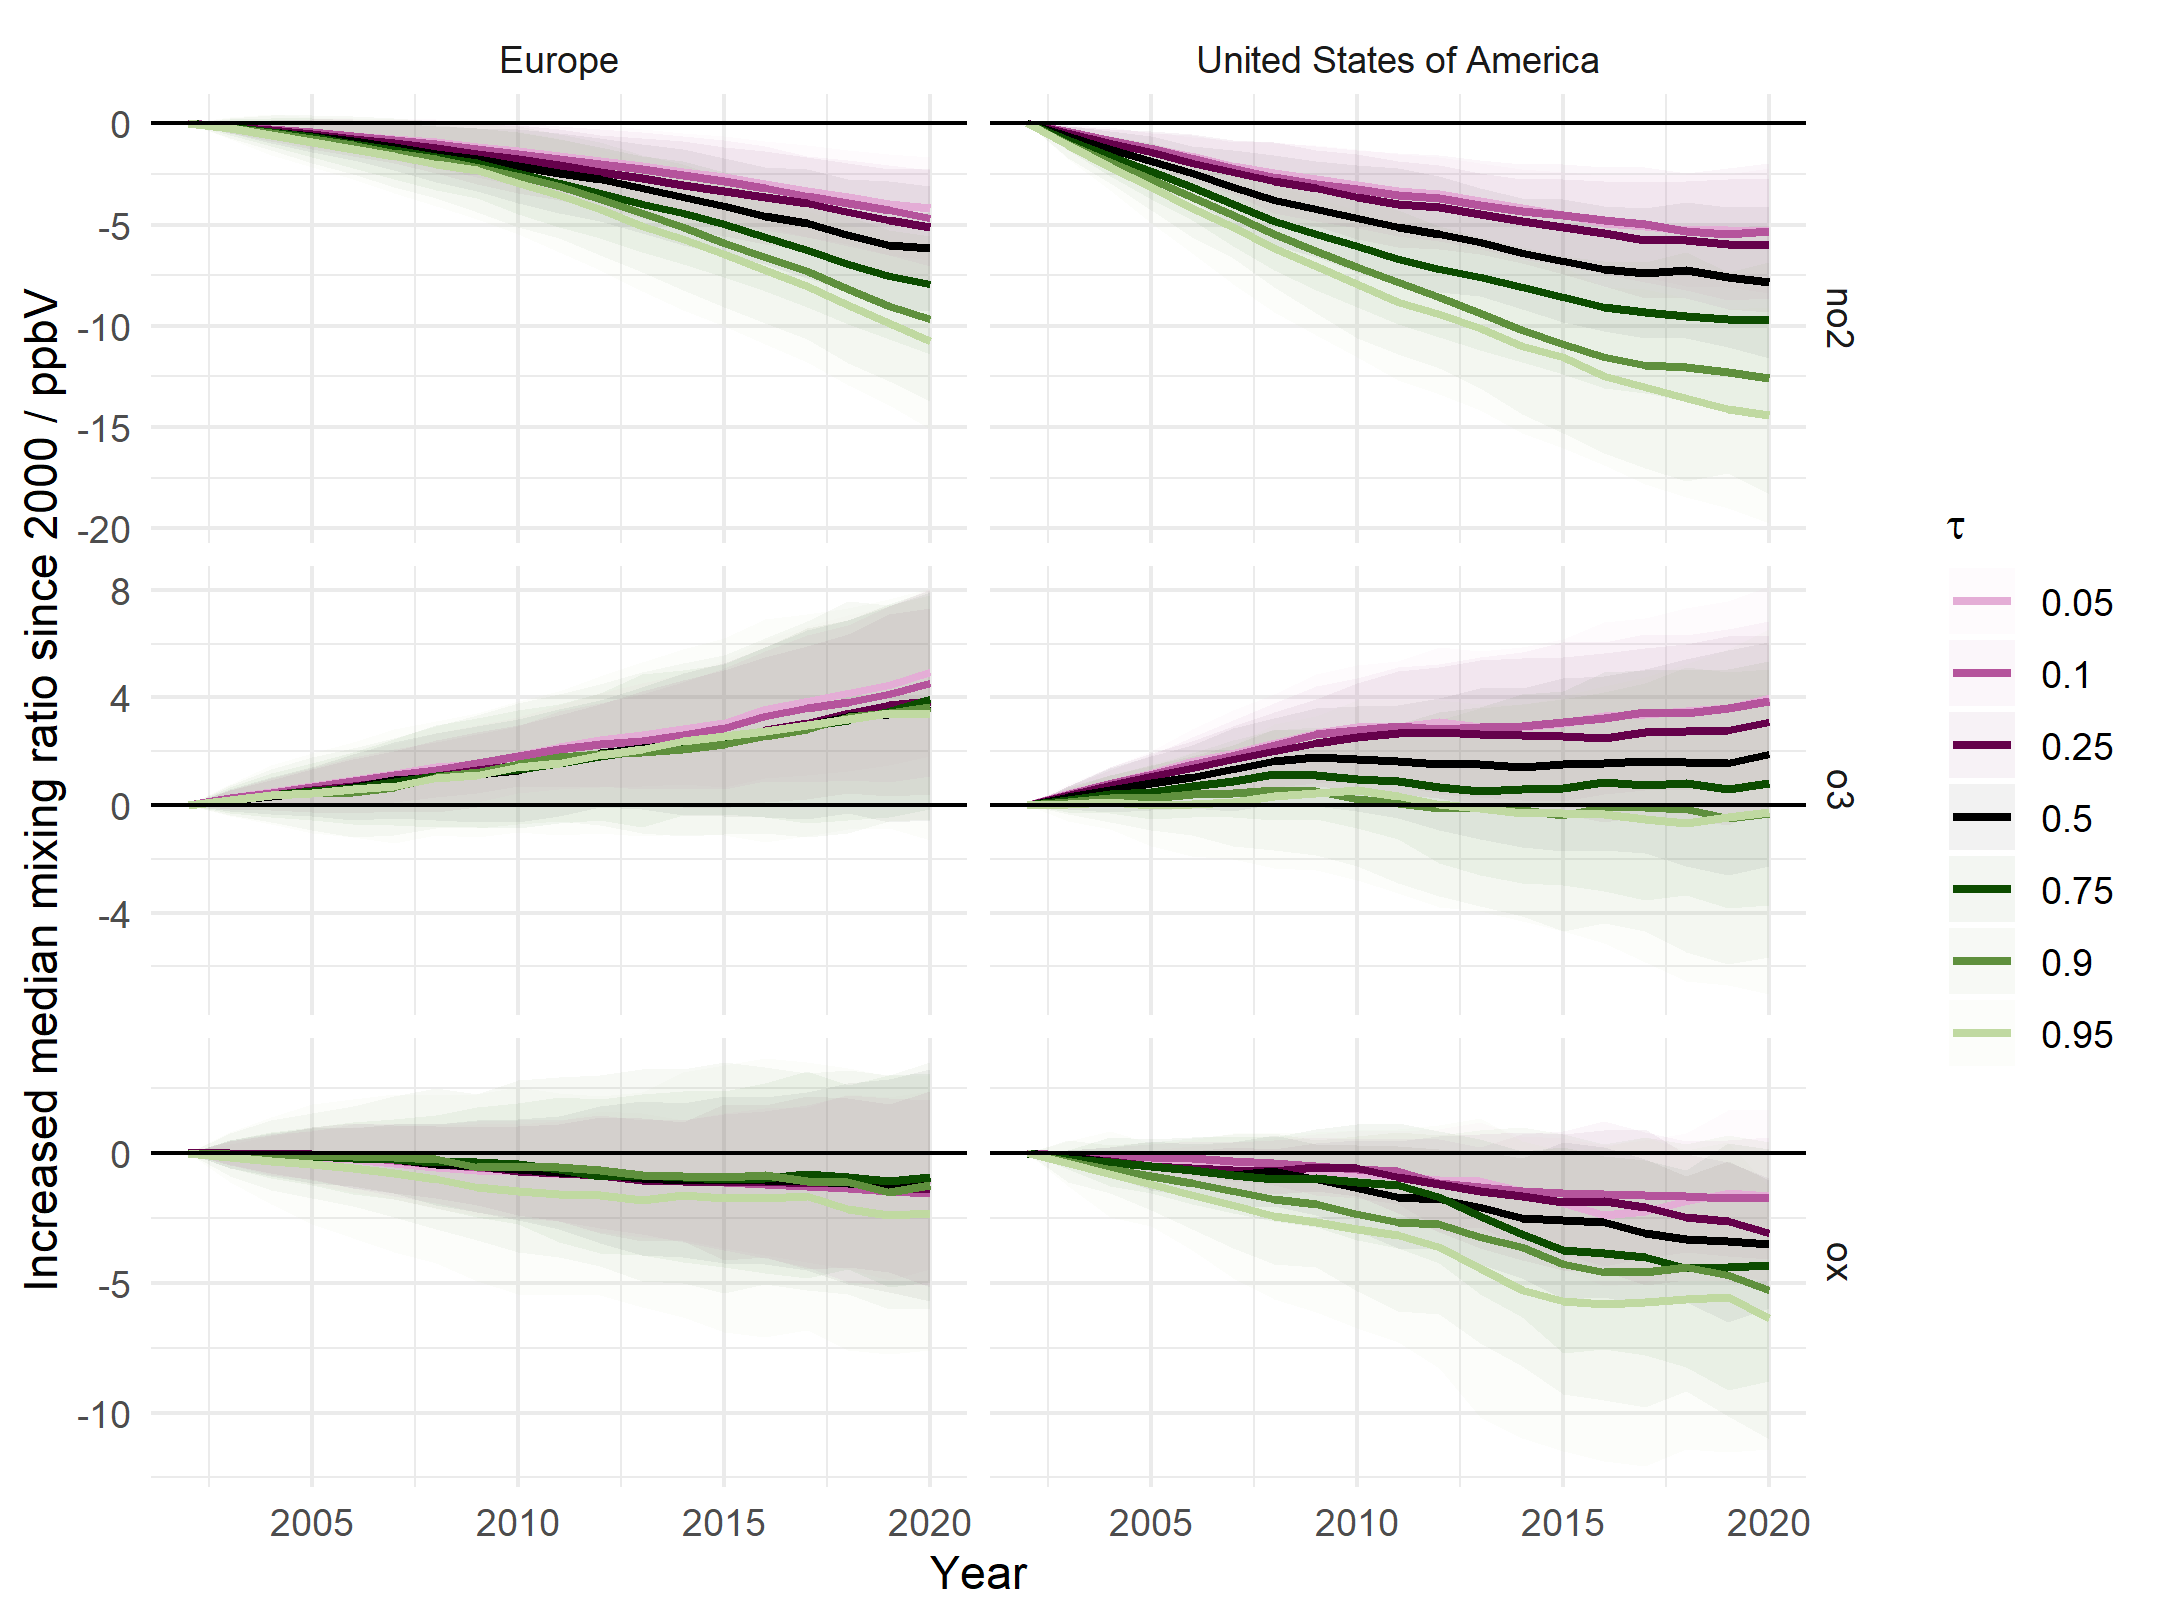
\includegraphics[width=12cm]{plots/fixed_median_slopes_per_tau_continent_name_absolute_change_with_mad_ribbon.png}
\caption{Absolute change in trendline-derived median NO2, O3 and Ox mixing ratios for Europe and the USA, coloured by trendline percentile. The shaded region represents the median absolute deviation.}
\label{median_slopes_per_tau_cont_name_absolute}
\end{figure*}

Taking a closer look at the annual magnitude and direction of the trends allows for a closer inspection of how o3 and no2 trends have changed between 2000 and 2021 for each percentile (Figure \ref{median_slopes_per_tau_cont_name_trends}). For Europe, all median O3 trends were positive for all percentiles. For higher percentiles (75th, 90th and 95th), the slope dropped sharply from ca. 0.54 ppbV yr-1 to ca 0.07 ppb yr-1 (95th percentile case) between 2000 and 2004. A smaller decrease in slope was observed for the lower percentiles (from ca. 0.35 ppb y-1 to 0.18 ppb yr-1 for the 5th percentile case). From 2005 onward, the slope in the o3 trend generally continued to increase up to 2021. In the lower percentile cases, the median slope returned to 2000-2002 levels in 2021. For the higher percentiles, the magnitude of the median slope was between ca. 0.29 - 0.46 ppb yr-1 lower in 2021 than 2000. In the USA, a larger spread in the changing median slopes was observed between different percentiles. Generally, and in contrast to Europe, the median slope in O3 steadily decreased between 2000 and 2014, before plateauing between 2014 to 2021. For the lower percentiles, the slope in o3 remained positive between 2000 and 2021, but reduced by ca. 0.34 ppb y-1 between 2000 and 2014 (5th percentile case). Trends in the higher percentiles were positive at the beginning of the century, with a transition to a negative trend observed for the 75th (in 2013), 90th and 95th (both in 2007) percentiles. In the 50th percentile case, median trends in O3 plateau around 0 ppb y-1 from 2012, indicating no overall direction of trend. Trends in NO2 in Europe and the USA between 2000 and 2021 are also contrasting. In both Europe and the USA, median trends remain negative between 2000 and 2021, indicating NO2 is decreasing in both cases, as observed in Figure X. However, the direction of the trend is different in each region. In Europe, the slope of the trend is becoming increasingly more negative with time, particularly for the higher percentile cases (reduction of ca. 0.72 ppb yr-1 for the 95th percentile case). However, in the USA the negative trends are becoming increasingly more positive (or less negative) between 2000 and 2021 (0.29 ppb y-1 higher, 95th percentile case). Interestingly, in both cases, although important changes in the direction of the trend are observed for O3 and NO2, there is no clear change in trend for Ox despite a clear reduction in its absolute median mixing ratio (Figure \ref{median_slopes_per_tau_cont_name_absolute}). For all percentiles, Ox trends are negative and consistent in magnitude per percentile. The exception to this is observed in Europe between 2000 - 2003 where the Ox trend switches sharply from being positive (ca. +1.16 ppb y-1, 95th percentile) to negative (-0.16 ppb y-1, 95th percentile). The Ox trend then remains negative, and consistently < 0.25 ppb y-1 for most percentiles (excluding the 95th percentile) between 2004 - 2021, and including the 95th percentile from 2009 onward.

\begin{figure*}[t]
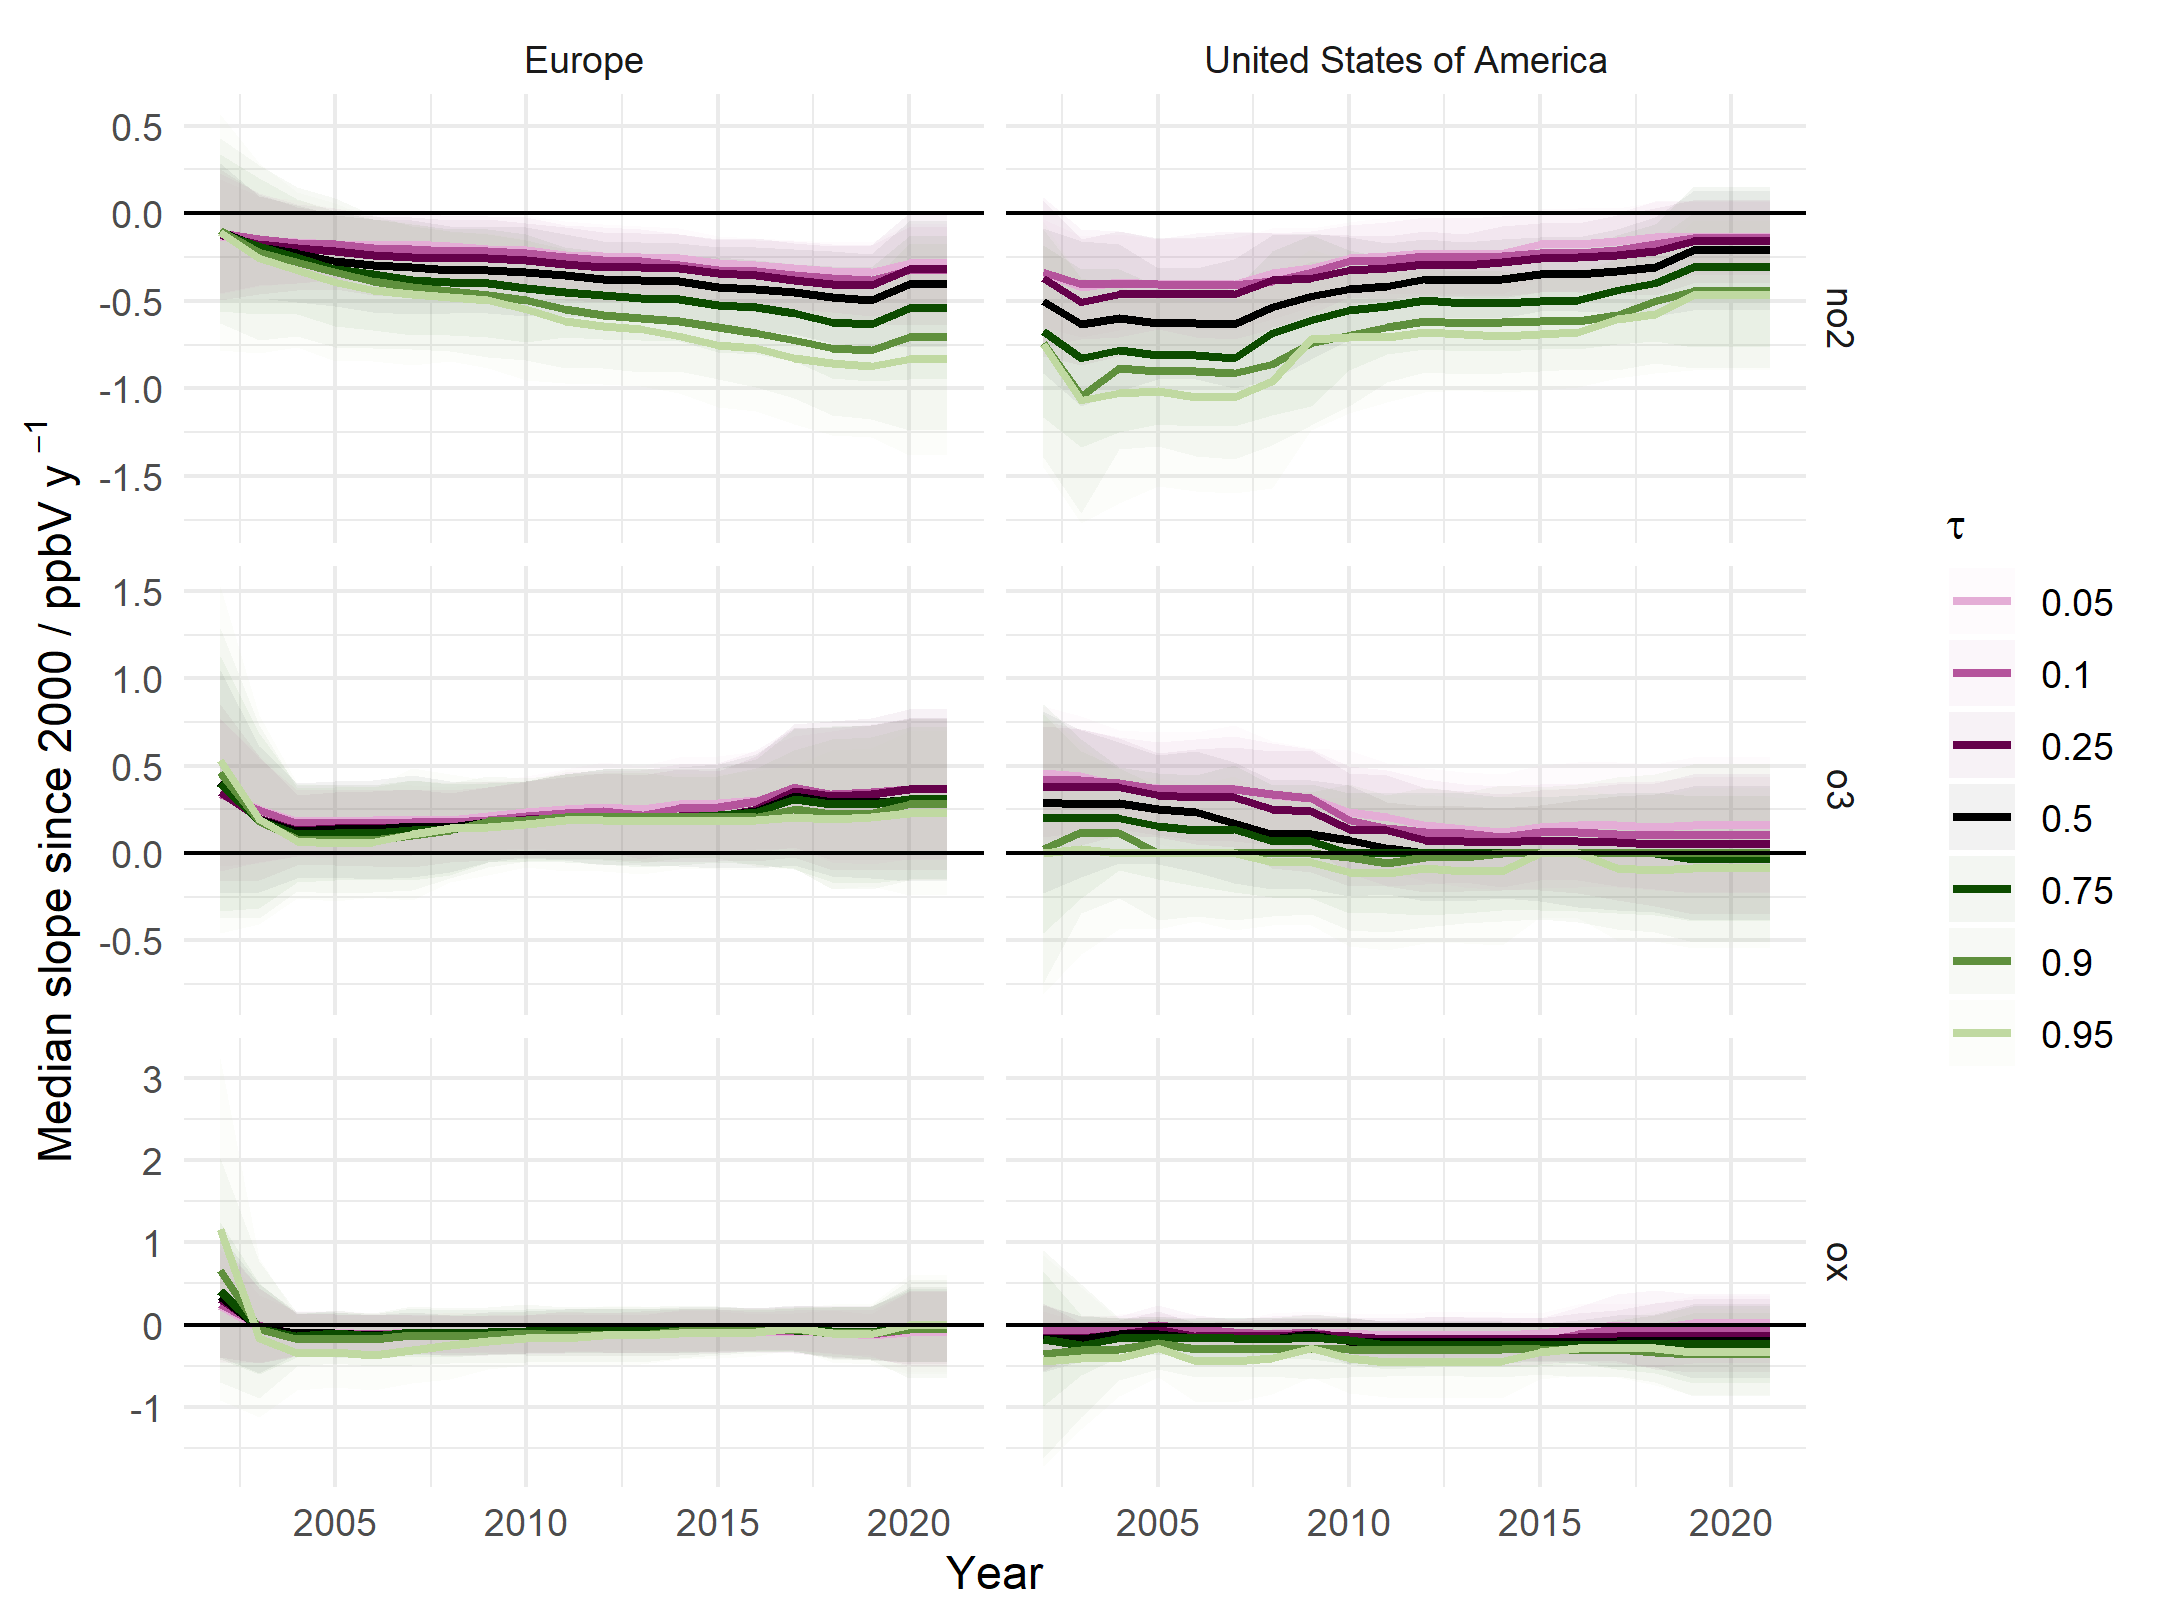
\includegraphics[width=12cm]{plots/fixed_median_slopes_per_tau_continent_name.png}
\caption{Median trendline slopes (ppb y-1) in NO2, O3 and Ox for Europe and the USA, coloured by trendline percentile. The shaded region represents the median absolute deviation.}
\label{median_slopes_per_tau_cont_name_trends}
\end{figure*}

\clearpage

\subsection{2020 In Europe}
TEXT

\section{Conclusion}  %% \conclusions[modified heading if necessary]
TEXT

%% The following commands are for the statements about the availability of data sets and/or software code corresponding to the manuscript.
%% It is strongly recommended to make use of these sections in case data sets and/or software code have been part of your research the article is based on.

\codeavailability{TEXT} %% use this section when having only software code available


\dataavailability{TEXT} %% use this section when having only data sets available


\codedataavailability{TEXT} %% use this section when having data sets and software code available


\sampleavailability{TEXT} %% use this section when having geoscientific samples available


\videosupplement{TEXT} %% use this section when having video supplements available


\appendix
\section{}    %% Appendix A

\subsection{}     %% Appendix A1, A2, etc.


\noappendix       %% use this to mark the end of the appendix section. Otherwise the figures might be numbered incorrectly (e.g. 10 instead of 1).

%% Regarding figures and tables in appendices, the following two options are possible depending on your general handling of figures and tables in the manuscript environment:

%% Option 1: If you sorted all figures and tables into the sections of the text, please also sort the appendix figures and appendix tables into the respective appendix sections.
%% They will be correctly named automatically.

%% Option 2: If you put all figures after the reference list, please insert appendix tables and figures after the normal tables and figures.
%% To rename them correctly to A1, A2, etc., please add the following commands in front of them:

\appendixfigures  %% needs to be added in front of appendix figures

\appendixtables   %% needs to be added in front of appendix tables

%% Please add \clearpage between each table and/or figure. Further guidelines on figures and tables can be found below.



\authorcontribution{TEXT} %% this section is mandatory

\competinginterests{TEXT} %% this section is mandatory even if you declare that no competing interests are present

\disclaimer{TEXT} %% optional section

\begin{acknowledgements}
TEXT
\end{acknowledgements}




%% REFERENCES

%% The reference list is compiled as follows:

\begin{thebibliography}{}

\bibitem[AUTHOR(YEAR)]{LABEL1}
REFERENCE 1

\bibitem[AUTHOR(YEAR)]{LABEL2}
REFERENCE 2

\end{thebibliography}

%% Since the Copernicus LaTeX package includes the BibTeX style file copernicus.bst,
%% authors experienced with BibTeX only have to include the following two lines:
%%
%% \bibliographystyle{copernicus}
%% \bibliography{example.bib}
%%
%% URLs and DOIs can be entered in your BibTeX file as:
%%
%% URL = {http://www.xyz.org/~jones/idx_g.htm}
%% DOI = {10.5194/xyz}


%% LITERATURE CITATIONS
%%
%% command                        & example result
%% \citet{jones90}|               & Jones et al. (1990)
%% \citep{jones90}|               & (Jones et al., 1990)
%% \citep{jones90,jones93}|       & (Jones et al., 1990, 1993)
%% \citep[p.~32]{jones90}|        & (Jones et al., 1990, p.~32)
%% \citep[e.g.,][]{jones90}|      & (e.g., Jones et al., 1990)
%% \citep[e.g.,][p.~32]{jones90}| & (e.g., Jones et al., 1990, p.~32)
%% \citeauthor{jones90}|          & Jones et al.
%% \citeyear{jones90}|            & 1990



%% FIGURES

%% When figures and tables are placed at the end of the MS (article in one-column style), please add \clearpage
%% between bibliography and first table and/or figure as well as between each table and/or figure.

% The figure files should be labelled correctly with Arabic numerals (e.g. fig01.jpg, fig02.png).


%% ONE-COLUMN FIGURES

%%f
%\begin{figure}[t]
%\includegraphics[width=8.3cm]{FILE NAME}
%\caption{TEXT}
%\end{figure}
%
%%% TWO-COLUMN FIGURES
%
%%f
%\begin{figure*}[t]
%\includegraphics[width=12cm]{FILE NAME}
%\caption{TEXT}
%\end{figure*}
%
%
%%% TABLES
%%%
%%% The different columns must be seperated with a & command and should
%%% end with \\ to identify the column brake.
%
%%% ONE-COLUMN TABLE
%
%%t
%\begin{table}[t]
%\caption{TEXT}
%\begin{tabular}{column = lcr}
%\tophline
%
%\middlehline
%
%\bottomhline
%\end{tabular}
%\belowtable{} % Table Footnotes
%\end{table}
%
%%% TWO-COLUMN TABLE
%
%%t
%\begin{table*}[t]
%\caption{TEXT}
%\begin{tabular}{column = lcr}
%\tophline
%
%\middlehline
%
%\bottomhline
%\end{tabular}
%\belowtable{} % Table Footnotes
%\end{table*}
%
%%% LANDSCAPE TABLE
%
%%t
%\begin{sidewaystable*}[t]
%\caption{TEXT}
%\begin{tabular}{column = lcr}
%\tophline
%
%\middlehline
%
%\bottomhline
%\end{tabular}
%\belowtable{} % Table Footnotes
%\end{sidewaystable*}
%
%
%%% MATHEMATICAL EXPRESSIONS
%
%%% All papers typeset by Copernicus Publications follow the math typesetting regulations
%%% given by the IUPAC Green Book (IUPAC: Quantities, Units and Symbols in Physical Chemistry,
%%% 2nd Edn., Blackwell Science, available at: http://old.iupac.org/publications/books/gbook/green_book_2ed.pdf, 1993).
%%%
%%% Physical quantities/variables are typeset in italic font (t for time, T for Temperature)
%%% Indices which are not defined are typeset in italic font (x, y, z, a, b, c)
%%% Items/objects which are defined are typeset in roman font (Car A, Car B)
%%% Descriptions/specifications which are defined by itself are typeset in roman font (abs, rel, ref, tot, net, ice)
%%% Abbreviations from 2 letters are typeset in roman font (RH, LAI)
%%% Vectors are identified in bold italic font using \vec{x}
%%% Matrices are identified in bold roman font
%%% Multiplication signs are typeset using the LaTeX commands \times (for vector products, grids, and exponential notations) or \cdot
%%% The character * should not be applied as mutliplication sign
%
%
%%% EQUATIONS
%
%%% Single-row equation
%
%\begin{equation}
%
%\end{equation}
%
%%% Multiline equation
%
%\begin{align}
%& 3 + 5 = 8\\
%& 3 + 5 = 8\\
%& 3 + 5 = 8
%\end{align}
%
%
%%% MATRICES
%
%\begin{matrix}
%x & y & z\\
%x & y & z\\
%x & y & z\\
%\end{matrix}
%
%
%%% ALGORITHM
%
%\begin{algorithm}
%\caption{...}
%\label{a1}
%\begin{algorithmic}
%...
%\end{algorithmic}
%\end{algorithm}
%
%
%%% CHEMICAL FORMULAS AND REACTIONS
%
%%% For formulas embedded in the text, please use \chem{}
%
%%% The reaction environment creates labels including the letter R, i.e. (R1), (R2), etc.
%
%\begin{reaction}
%%% \rightarrow should be used for normal (one-way) chemical reactions
%%% \rightleftharpoons should be used for equilibria
%%% \leftrightarrow should be used for resonance structures
%\end{reaction}
%
%
%%% PHYSICAL UNITS
%%%
%%% Please use \unit{} and apply the exponential notation


\end{document}
